\documentclass[a4paper,12pt]{book}            % Book class with paper size and font

% Essential packages
\usepackage[utf8]{inputenc}                     % UTF-8 encoding
\usepackage[T1]{fontenc}                        % Output font encoding for proper Spanish chars
\usepackage[spanish]{babel}                     % Spanish language
\usepackage{amsmath,amssymb,amsthm}             % For math
\usepackage{graphicx}                           % For images
\usepackage{listings}                           % For code snippets
\usepackage{tikz}                               % Required for pgfgantt
\usepackage{pgfplots}                           % For plots and charts
\pgfplotsset{compat=1.18}                       % Set pgfplots compatibility level

% For multipage tables
\usepackage{longtable}
\usepackage{hyperref}                           % For clickable links and references
\usepackage{bookmark}                           % For bookmarks
\usepackage{makeidx}
\usepackage{geometry}                           % For margins
\usepackage{fancyhdr}                           % Headers and footers
\usepackage{parskip}                            % Spacing between paragraphs
\usepackage{xcolor}                             % For colors
\usepackage{pgfgantt}                           % For Gantt charts
\usepackage{authoraftertitle}                   % For author and title
\usepackage{lipsum}                             % For dummy text
\usepackage{nomencl}                            % For nomenclature
\usepackage{natbib}                             % For bibliography
\usepackage{subcaption}                         % For subfigures

\makenomenclature
\makeindex
\bibliographystyle{apalike}                     % APA style for bibliography
\setlength{\headheight}{14.49998pt}             % Adjust head height

\title{Neural Analytics: una herramienta software basada en redes neuronales de procesado de EEGs}
\author{Sergio Martínez Aznar}                  

% Header and footer configuration
\pagestyle{fancy}
\fancyhf{}
\fancyhead[L]{Neural Analytics}                 % Left header
\setlength{\headwidth}{16cm}                    % Header width
\fancyhead[R]{\thepage}                         % Right header (page number)
\fancyfoot[C]{Autor: Sergio Martinez Aznar}     % Centered footer
\geometry{margin=2.5cm}                         % Margin settings

% Code configuration
\lstset{
    basicstyle=\ttfamily\small,                 % Font style
    numbers=left,                               % Line numbers
    numberstyle=\tiny,                          % Number size
    stepnumber=1,                               % Step number
    frame=single,                               % Box around code
    breaklines=true,                            % Break long lines
    captionpos=b,                               % Title position
    language=Python                             % Default language
}

\begin{document}

% Title
\newgeometry{margin=0in}


% Alturas ajustadas para que encajen en una sola página
\newcommand{\blockheight}{21cm} % Altura del bloque amarillo pastel
\newcommand{\footerheight}{8.3cm} % Altura del bloque negro
\fontfamily{phv}\selectfont % Start Helvetica font

% Bloque amarillo pastel
\noindent
\colorbox[HTML]{fef193}{ % Color amarillo pastel
    \parbox[b][\blockheight][c]{\textwidth}{ % Bloque del tamaño adecuado

        \begin{center}
            {
                \Huge\textbf{\MyTitle\\[0.2cm]}
            } 
            {\Large Grado en Ingenieria Informática} \\
        \end{center}
    }
}\vspace{-8pt}% Elimina el espacio entre bloques

% Bloque negro
\noindent
\colorbox{black}{
    \parbox[b][\footerheight][c]{\textwidth}{ % Bloque del tamaño adecuado
        \color{white} % Texto en color blanco
        \begin{center}
            \begin{tabular}{p{0.7\textwidth}c}
                {\large\textbf{Trabajo Fin de Grado}} \\[0.5cm]
                \textbf{Autor:} \MyAuthor \\[0.2cm]
                \textbf{Tutor/es:} Jordi Linares \\[0.2cm]
                \textbf{Curso Académico:} 2024/2025 \\[0.2cm]
                \textbf{Fecha de Depósito:} \today
                &
                \raisebox{-0.1\height}{\includegraphics[height=1.5cm]{./assets/logo_universidad.png}}
            
            \end{tabular}
        \end{center}
    }
}

\restoregeometry
\fontfamily{\familydefault}\selectfont % Restore default font

% Giving thanks
\newpage
\thispagestyle{empty}
\vspace*{\fill}
\textit{Para aquellos que soñaron con alguna vez con volar alto, y lo arriesgaron todo.}
\vspace*{\fill}

% Introduction and Abstract
\frontmatter
    % Abstracts
    % Chapter 1: Abstract
\chapter*{Resumen}
\addcontentsline{toc}{chapter}{Resumen}

Este proyecto presenta el desarrollo de un sistema de control domótico basado en interfaces cerebro-computadora (BCI). El objetivo principal es implementar un sistema no invasivo que permita el control mental de dispositivos de iluminación inteligente, específicamente bombillas TP-Link Tapo.

El sistema utiliza la diadema Brainbit como dispositivo de adquisición de señales electroencefalográficas (EEG), procesando estas señales mediante una arquitectura de software que combina PyTorch para el entrenamiento de modelos de aprendizaje profundo y Rust para el desarrollo del motor de inferencia. 

El marco teórico aborda el desarrollo de un modelo de clasificación basado en señales EEG, explorando técnicas de procesamiento de señales y aprendizaje automático para la interpretación precisa de patrones cerebrales. Además, se profundiza en los requisitos técnicos y normativos necesarios para el desarrollo de dispositivos médicos, con especial énfasis en el estándar IEC 62304 para procesos del ciclo de vida del software de dispositivos médicos, y la implementación de sistemas operativos en tiempo real (RTOS) para garantizar la fiabilidad y seguridad del sistema.

La solución propuesta integra tecnologías modernas de procesamiento de señales cerebrales con sistemas de domótica, creando una interfaz natural e intuitiva para el control del entorno doméstico. Este proyecto representa un paso hacia la democratización de las interfaces cerebro-computadora en aplicaciones cotidianas.

\vspace{0.5cm}
\noindent\textbf{Palabras clave:} Interfaz cerebro-computadora, BCI, Domótica, Aprendizaje profundo, Rust, PyTorch, EEG, RTOS, Certificación médica


    % Chapter 1: Abstract
\chapter*{Abstract}
\addcontentsline{toc}{chapter}{Abstract}

This project presents the development of a home automation control system based on brain-computer interfaces (BCI). The main objective is to implement a non-invasive system that enables the integration of brain signals with smart lighting devices, specifically TP-Link Tapo bulbs.

The system uses the Brainbit headband as an electroencephalographic (EEG) signal acquisition device, processing these signals through a software architecture that combines PyTorch for training deep learning models and Rust for the development of the inference engine.

The theoretical framework addresses the development of a classification model based on EEG signals, exploring signal processing and machine learning techniques for accurate interpretation of brain patterns. Additionally, it delves into the technical and regulatory requirements necessary for medical device development, with special emphasis on the IEC 62304 standard for medical device software life cycle processes, and the implementation of real-time operating systems (RTOS) to ensure system reliability and safety.

The proposed solution integrates modern brain signal processing technologies with home automation systems, creating a natural and intuitive interface for controlling the home environment. This project represents a step towards the democratization of brain-computer interfaces in everyday applications.

\vspace{0.5cm}
\noindent\textbf{Keywords:} Brain-computer interface, BCI, Home automation, Deep learning, Rust, PyTorch, EEG, RTOS, Medical certification

    % Tables of Contents and Figures
    \include{chapters/chapter_aux/TableOfContents}
    \include{chapters/chapter_aux/TableOfFigures}
    \include{chapters/chapter_aux/TableOfNotations}

% Chapters
\mainmatter

    % Chapter 2: Introduction
\chapter*{Introduction}
\addcontentsline{toc}{chapter}{Introduction}

\lipsum[1-8]

    \part{Marco Teórico}
        \chapter{Normativa UNE-EN 62304}\label{ch:regulatory_framework}

La norma \textbf{UNE-EN 62304:2007/A1:2016} \cite{UNE-EN-62304} es la versión española de la norma \textbf{IEC 62304:2006/A1:2015}, adoptada como norma europea EN 62304:2006/A1:2015. Esta normativa establece los requisitos para los \textbf{procesos del ciclo de vida del software} en \textbf{dispositivos médicos}, asegurando su desarrollo, mantenimiento y gestión de riesgos de acuerdo con estándares internacionales.

\section{Objetivo y Alcance}
El propósito de la UNE-EN 62304 \cite{UNE-EN-62304} es definir un marco normativo para la \textbf{gestión del ciclo de vida del software} en dispositivos médicos, asegurando su seguridad y eficacia. 

Esta norma se aplica a:
\begin{itemize}
    \item \textbf{Software que es un dispositivo médico en sí mismo.}
    \item \textbf{Software embebido en dispositivos médicos.}
    \item \textbf{Software utilizado en entornos médicos para diagnóstico, monitoreo o tratamiento.}
\end{itemize}

El estándar establece \textbf{procesos y actividades} que los fabricantes deben seguir, incluyendo:
\begin{itemize}
    \item Planificación del desarrollo del software.
    \item Análisis de requisitos y arquitectura del software.
    \item Implementación, integración, pruebas y verificación.
    \item Gestión del mantenimiento y resolución de problemas.
    \item Gestión del riesgo asociado al software.
    \item Gestión de la configuración y cambios.
\end{itemize}

\newpage
\section{Clasificación del Software}
La norma clasifica el software en \textbf{tres niveles de seguridad} según el riesgo que pueda representar para el paciente o el operador:

\begin{itemize}
    \item \textbf{Clase A}: El software no puede causar daño en ninguna circunstancia.
    \item \textbf{Clase B}: El software puede contribuir a una situación peligrosa, pero el daño potencial es \textbf{no serio}.
    \item \textbf{Clase C}: El software puede contribuir a una situación peligrosa con \textbf{riesgo de daño serio o muerte}.
\end{itemize}

\section{Cumplimiento y Aplicación durante el proyecto}
Para garantizar el cumplimiento de la UNE-EN 62304 \cite{UNE-EN-62304} en este trabajo, se seguirá un enfoque basado en la \textbf{gestión del ciclo de vida del software} y la evaluación de riesgos. Se adoptarán buenas prácticas de ingeniería de software y se documentarán las actividades necesarias para cumplir con los requisitos de seguridad y calidad establecidos por la normativa.

En este proyecto, utilizaremos un \textbf{modelo de desarrollo iterativo e incremental} inspirado en metodologías ágiles como Scrum, adaptado a las necesidades específicas del desarrollo de software médico. Este enfoque nos permitirá una mayor flexibilidad y capacidad de adaptación a los cambios, así como una entrega continua de valor al cliente.

Considerando que el sistema únicamente controla el encendido y apagado de una bombilla inteligente TP-Link Tapo de manera remota, hemos clasificado el software como de \textbf{Clase A}. Esta clasificación se justifica porque el software no puede causar daño al usuario en ninguna circunstancia, ya que:
\begin{itemize}
    \item La diadema BrainBit es un dispositivo no invasivo de lectura pasiva
    \item El control se realiza sobre una bombilla doméstica de baja tensión
    \item No hay interacción directa con sistemas críticos o vitales
\end{itemize}

A pesar de esta clasificación de bajo riesgo, mantendremos buenas prácticas de desarrollo y documentación para asegurar la calidad del software.

Dado que esta normativa es un \textbf{requisito esencial} para el desarrollo de software en el mercado sanitario español y europeo, su correcta implementación garantizará la viabilidad del producto en entornos clínicos y su aceptación por parte de los organismos reguladores.
        \chapter{Regiones implicadas del cerebro}\label{ch:brain_regions}

\section{Introducción a las Regiones Cerebrales Funcionales}

El cerebro humano es un sistema altamente organizado en el que diferentes regiones trabajan de manera especializada pero interconectada para procesar la información y generar respuestas conductuales adecuadas. Como indican en su libro "Principios de Neurociencia" los autores Kandel, Jessell y Schwartz (\citeyear{Kandel_Jessell_Schwartz_2001}), el estudio de la neurociencia ha demostrado que la división funcional del cerebro permite analizar la forma en que los procesos perceptivos, cognitivos y emocionales emergen de la actividad neuronal distribuida. En este proyecto, nos enfocamos en dos regiones clave para la percepción y la memoria del color: el lóbulo occipital y el lóbulo temporal. 

Utilizando un sistema BCI basado en EEG, empleamos electrodos en ubicaciones específicas del sistema internacional 10-20: O1 y O2 en el lóbulo occipital, responsables del procesamiento primario de la información visual, y T3 y T4 en el lóbulo temporal, donde la información visual se asocia con memorias previas y respuestas emocionales. 

Gracias a esta organización funcional, podemos estudiar la relación entre percepción e imaginación del color, explorando su impacto en la memoria y la experiencia subjetiva.

\newpage

\section{El Lóbulo Temporal y la Memoria Visual}

El lóbulo temporal es crucial en la memoria visual y la asociación semántica de colores. Los electrodos T3 y T4 captan la actividad relacionada con:

\begin{itemize}
    \item \textbf{Hipocampo:} Responsable de la consolidación de memorias visuales y asociaciones cromáticas.
    \item \textbf{Corteza temporal medial:} Procesa la identificación y categoría de los colores.
    \item \textbf{Amígdala:} Relaciona el color con respuestas emocionales, modulando el impacto afectivo de los colores percibidos o imaginados.
    \item \textbf{Corteza entorrinal:} Conecta el hipocampo con otras áreas corticales, permitiendo que las asociaciones cromáticas se integren en experiencias más complejas.
\end{itemize}

Cuando una persona recuerda un color, T3 y T4 reflejan la activación de estos circuitos, permitiendo analizar la relación entre percepción visual y memoria. Estudios como los de Squire y Zola-Morgan (\citeyear{Squire_Zola_Morgan_1991}) han demostrado que lesiones en el lóbulo temporal pueden afectar la capacidad de recuperar memorias visuales, lo que refuerza su papel en el almacenamiento de información sensorial.

\section{El Lóbulo Occipital y la Percepción del Color}

El lóbulo occipital es la principal región del cerebro para el procesamiento de la información visual.  Los electrodos O1 y O2 capturan la actividad en:

\begin{itemize}
    \item \textbf{Corteza visual primaria (V1):} Primer procesamiento del color y detección de longitudes de onda. \footnote{Es importante distinguir entre O1/O2, que son las \textit{posiciones de los electrodos} según el sistema internacional 10-20, y V1/V4, que son \textit{áreas funcionales del córtex visual} (designaciones de Brodmann) cuya actividad es registrada por dichos electrodos.}
    
    \item \textbf{V4 (corteza visual asociativa):} Especializada en la interpretación y categorización de colores, estableciendo una conexión funcional con las áreas temporales para asignar significados semánticos.
\end{itemize}

Estudios como los de Brouwer y Heeger (\citeyear{Brouwer_Heeger_2013}) han demostrado que la actividad en V4 puede ser utilizada para clasificar diferentes colores percibidos o imaginados, lo que refuerza la validez de nuestros electrodos O1 y O2 para el análisis de patrones cromáticos en EEG.

\newpage

\section{Integración entre Memoria y Percepción}
El procesamiento del color en el cerebro, simplificándolo al absurdo, sigue un flujo distribuido:
\begin{enumerate}
    \item O1/O2 detectan y analizan las características del color percibido o imaginado.
    \item La información es enviada a T3/T4 para su comparación con recuerdos previos y asociaciones emocionales.
    \item Se generan asociaciones semánticas y afectivas, determinando la experiencia subjetiva del color.
\end{enumerate}

Estudios como los de Rissman y Wagner (\citeyear{Rissman_Wagner_2012}) han mostrado que patrones de activación en el lóbulo temporal pueden predecir si un individuo reconoce un color previamente visto, lo que refuerza la idea de que los recuerdos cromáticos tienen una representación neural clara.

\section{Aplicaciones en Interfaces Cerebro-Computadora}

La integración de la percepción y la memoria del color en un sistema BCI tiene varias aplicaciones potenciales:

\begin{itemize}
    \item Diferenciar entre percepción real e imaginada de un color.
    \item Implementar sistemas BCI basados en selección cromática.
    \item Explorar la relación entre color, memoria y emociones para aplicaciones en neurotecnología.
\end{itemize}

De este modo, podemos exploar mediante una interfaz cerebro-computadora cómo la percepción y la memoria del color se integran en la experiencia subjetiva, permitiendo así que pueda ser interpretado por un computador y que este pueda realizar acciones en función de la información recibida.

\section{Aplicaciones durante este proyecto}
Los electrodos O1, O2, T3 y T4 capturan información clave sobre la percepción y la memoria del color. Su combinación permite analizar la reconstrucción mental de colores y su impacto en la experiencia subjetiva, formando la base de nuestro sistema BCI. La inclusión de referencias a trabajos clave refuerza la validez del enfoque adoptado en este estudio.
        \chapter{Sistemas operativos en Tiempo Real}\label{ch:real_time_oses}

Los sistemas operativos en tiempo real (RTOS) \cite{Siewert_Pratt_2016} son una rama del software que busca garantizar ejecución de tareas en plazos temporales específicos, pues el concepto mismo de computación en tiempo real nace de la necesidad de procesar y responder a eventos externos con restricciones de tiempo bien definidas. Entonces, la corrección del sistema no solo depende de la lógica de los resultados, sino también del momento exacto en que estos se producen.

Las características que diferencian a un RTOS de sistemas operativos convencionales son:

\begin{itemize}
    \item \textbf{Determinismo}: Propiedad fundamental donde dada una entrada y estado inicial, nos va a devolver siempre la misma salida en tiempos predecibles.
    \item \textbf{Concurrencia}: Capacidad para gestionar varias tareas en espacios temporales limitados sin comprometer plazos críticos.
    \item \textbf{Interrupciones}: Mecanismos para responder a eventos externos de forma rápida y predecible.
    \item \textbf{Planificación}: Algoritmos que controlan el orden y tiempo de ejecución de tareas según su criticidad temporal.
\end{itemize}

En el campo de los sistemas embebidos, un RTOS actúa como intermediario entre el hardware y las operaciones de control. El ejemplo clásico de los controladores de vuelo en aeronaves es quizá el más ilustrativo, donde cualquier fallo en los tiempos de respuesta puede tener efectos catastróficos. Estos sistemas aparecen también en satélites artificiales, que suelen tener varios RTOS ejecutando en paralelo para controlar tanto las funciones del vehículo como los instrumentos científicos, todo trabajando de forma armónica.

Al investigar aplicaciones de RTOS, he encontrado muchos sectores donde son vitales: en entornos industriales para control de procesos críticos; en aviónica para sistemas de navegación (con certificaciones súper estrictas); en defensa para sistemas de radar; y —importante para este proyecto— en el sector médico, donde dispositivos como marcapasos, respiradores y bombas de infusión necesitan respuestas predecibles para garantizar seguridad del paciente.

\newpage
\section{Taxonomía de Sistemas en Tiempo Real}
    La clasificación básica de RTOS se basa en la criticidad de sus restricciones temporales. Esta taxonomía viene de Liu y Layland en 1973 \cite{Siewert_Pratt_2016} y distingue principalmente entre sistemas estrictos (\textit{hard real-time}) y flexibles (\textit{soft real-time}). Mi entendimiento de estas categorías cambió bastante al ver aplicaciones reales, pues la línea entre ambas no es tan clara como dicen los libros.

    \subsection{Sistemas de Tiempo Real Estricto}
        Los sistemas estrictos (\textbf{hard real-time}) no toleran ninguna desviación en sus plazos temporales. Si se incumple un plazo, se considera un fallo crítico del sistema —algo que da bastante miedo cuando piensas en sus aplicaciones en entornos críticos. Su comportamiento se puede expresar matemáticamente como:

        \begin{figure}[h!]
            \centering
            \begin{equation}
                \forall t \in T: R(t) \leq D(t)
            \end{equation}
            \caption{Ecuación de sistemas de tiempo real estricto.}
            \label{fig:hard_real_time_equation}
        \end{figure}

        donde $R(t)$ es el tiempo de respuesta y $D(t)$ el plazo máximo permitido.

        Algunos de los casos de uso más comunes para estos sistemas son:
        \begin{itemize}
            \item \textbf{Control nuclear}: Donde la precisión temporal es crítica para la seguridad
            \item \textbf{Sistemas ABS}: Responden en microsegundos para evitar accidentes
            \item \textbf{Robótica quirúrgica}: Necesitan sincronización precisa durante operaciones
        \end{itemize}

    La implementación requiere algoritmos \textbf{preemptivos} con prioridades estáticas, donde el tiempo máximo de ejecución debe ser predecible. Normalmente usan Rate Monotonic (RM) o Earliest Deadline First (EDF). Cuando intenté implementar esto en mis pruebas iniciales, me di cuenta que garantizar determinismo absoluto en hardware normal es casi imposible y me tocó replantear algunas decisiones.

    \newpage
    \subsection{Sistemas de Tiempo Real Flexible}
        Los sistemas flexibles (\textbf{soft real-time}) toleran cierta variabilidad en sus plazos, funcionando con un modelo estadístico. Es algo así como:

        \begin{figure}[h!]
            \centering
            \begin{equation}
                P(R(t) \leq D(t)) \geq p_{min}
            \end{equation}            \caption{Ecuación de sistemas de tiempo real flexible.}
            \label{fig:soft_real_time_equation}
        \end{figure}

        donde $p_{min}$ es el nivel mínimo aceptable de cumplimiento.

        Las aplicaciones más comunes son:
        \begin{itemize}
            \item \textbf{Streaming multimedia}: Perder algunos frames de vez en cuando no arruina la experiencia
            \item \textbf{Redes de monitorización}: Toleran retrasos ocasionales en actualizar datos
            \item \textbf{Trading algorítmico}: Les importa más el rendimiento promedio que garantías absolutas
        \end{itemize}

        Estos sistemas usan planificadores basados en \textbf{tiempo compartido} con prioridades dinámicas. Para mi interfaz cerebro-computadora, este enfoque fue mejor, ya que pequeñas variaciones en los tiempos no afectan mucho la experiencia. Después de analizar bien los requisitos temporales, vi claramente que este modelo no solo cumplía lo necesario, sino que ofrecía mejor balance entre complejidad y prestaciones.

    \subsection{Consideraciones de Implementación}
        La decisión entre sistemas estrictos o flexibles depende de varios factores:
        \begin{itemize}
            \item \textbf{Riesgos}: ¿Qué pasa si se incumple un plazo temporal?
            \item \textbf{Hardware disponible}: Limitaciones de procesamiento y memoria
            \item \textbf{Presupuesto}: Balance entre garantías temporales y complejidad
            \item \textbf{Regulaciones}: Requisitos de certificación según donde se use
        \end{itemize}

\newpage
\section{Soluciones Comerciales para Hard Real-Time}

    \subsection{VxWorks (Wind River Systems)}
        VxWorks es el referente en sistemas embebidos críticos, especialmente en aviónica, aeroespacial y médico. Cuando empecé a estudiarlo, su documentación me pareció abrumadora. Sus características principales:

        \subsubsection{Certificaciones y Normativas}
            \begin{itemize}
                \item DO-178C Level A para sistemas aeroespaciales
                \item IEC 62304 para dispositivos médicos
                \item ISO 26262 ASIL D para automoción
            \end{itemize}
        \subsubsection{Características Técnicas}
            \begin{itemize}
                \item \textbf{Kernel}: Microkernel determinista con latencias $\le$ 50 ns
                \item \textbf{Memoria}: MMU con protección y aislamiento
                \item \textbf{Scheduler}: 256 niveles de prioridad y herencia
                \item \textbf{IPC}: Comunicación con latencia determinista
                \item \textbf{Multiproceso}: Soporte para SMP y AMP con aislamiento
            \end{itemize}

        Al evaluar VxWorks me impresionó ver dónde se usa —desde rovers de Marte hasta dispositivos médicos certificados. Pero los costes de licencia para obtener un SDK personalizado eran prohibitivos para un proyecto que está en fase de prototipo.

    \newpage
    \subsection{QNX Neutrino (BlackBerry)}
        QNX Neutrino, que compró BlackBerry en 2010, destaca por su microkernel distribuido y fiabilidad. Es curioso que BlackBerry, después de casi desaparecer del mercado de móviles, mantenga este producto tecnológico tan avanzado:

        \subsubsection{Arquitectura}
            \begin{itemize}
                \item \textbf{Microkernel}: Núcleo muy pequeño, menos de 100KB
                \item \textbf{Servicios}: Arquitectura modular en espacio de usuario
                \item \textbf{IPC}: Mensajería con mecanismo copy-on-write
                \item \textbf{Recuperación}: Reinicio de componentes sin afectar al sistema
            \end{itemize}

        \subsubsection{Características Avanzadas}
            \begin{itemize}
                \item \textbf{Tiempo Real}: Latencias garantizadas $\le$ 100 $\mu$s
                \item \textbf{Seguridad}: Modelo de seguridad con ASLR
                \item \textbf{Certificaciones}: IEC 61508 SIL3, IEC 62304 Clase C
            \end{itemize}

        QNX me gustó mucho por su uso en dispositivos médicos. Su problema principal no fue tanto el coste —BlackBerry tiene licencias para desarrollo— sino que no tiene buen soporte para Rust, lo que complicaba integrar las librerías que consumía este proyecto. Después de tratar de hacerlo funcionar, decidí que no valía la pena invertir más tiempo y dejé de lado esta opción.

    \newpage
    \subsection{Zephyr RTOS (Linux Foundation)}
        Zephyr es la alternativa open-source para sistemas embebidos críticos. Este proyecto, inicialmente iniciado por Wind River y más adelante donado a la Linux Foundation, ha crecido rápidamente y tiene un ecosistema de desarrolladores muy activo. Me pareció una opción interesante para el prototipo:

        \subsubsection{Diseño y Arquitectura}
            \begin{itemize}
                \item \textbf{Kernel}: Configurable como monolítico o microkernel
                \item \textbf{Tamaño}: Desde 8KB hasta 512KB según configuración
                \item \textbf{Scheduler}: Hasta 32 niveles de prioridad
                \item \textbf{Certificación}: En proceso para IEC 61508 SIL 3/4
            \end{itemize}

        \subsubsection{Características Destacadas}
            \begin{itemize}
                \item \textbf{Drivers}: Más de 350 controladores para periféricos
                \item \textbf{Redes}: Soporte para protocolos IoT (BLE, Thread, LoRaWAN)
                \item \textbf{Seguridad}: Subsistema con aislamiento
                \item \textbf{Desarrollo}: Herramientas de depuración avanzadas
            \end{itemize}

        Aunque Zephyr era atractivo y sin coste económico, tenía también las complicaciones del soporte de librerías en Rust. Sin embargo, dadas sus características, preferí mirar otras opciones que pudieran contar con el núcleo de Linux y así aprovechar el ecosistema de librerías que ya tenía.

\newpage
\section{Soluciones Comerciales para Soft Real-Time}
    \subsection{Wind River Linux (Wind River Systems)}
        Wind River Linux es una solución comercial basada en Yocto para sistemas con requisitos temporales flexibles. Cuando la descubrí, me pareció una versión más accesible de VxWorks, con enfoque más moderno:

        \subsubsection{Características Principales}
            \begin{itemize}
                \item \textbf{Base}: Kernel Linux 5.10 LTS con parche PREEMPT\_RT
                \item \textbf{Certificaciones}: ISO 9001:2015 y precertificación IEC 62304
                \item \textbf{Seguridad}: Monitorización de vulnerabilidades y mitigación
                \item \textbf{Conformidad}: Documentación SBOM y Open Chain 2.1
            \end{itemize}

        \subsubsection{Capacidades Industriales}
            \begin{itemize}
                \item \textbf{Soporte}: Mantenimiento garantizado 5 años, extensible
                \item \textbf{Actualizaciones}: Sistema OTA mediante OSTree
                \item \textbf{Validación}: Más de 60.000 tests automatizados
                \item \textbf{Servicios}: Soporte técnico y consultoría
            \end{itemize}

        Al principio consideré seriamente Wind River Linux por su precertificación IEC 62304, importante para dispositivos médicos. Pero los costes de licencia y soporte eran demasiado altos para esta fase del proyecto, así que busqué opté por una alternativa más económica para diseñar el prototipo.

    \newpage
    \subsection{Poky Linux (Proyecto Yocto)}
        Poky es la distribución de referencia del Proyecto Yocto para sistemas Linux embebidos con capacidades de tiempo real flexible. Cuando empecé a usarlo, me pareció muy flexible, aunque aprender a usarlo fue más complicado de lo que esperaba:

        \subsubsection{Características Técnicas}
            \begin{itemize}
                \item \textbf{Kernel}: Linux con parche PREEMPT\_RT
                \item \textbf{Tiempo Real}: Latencias configurables según necesidades
                \item \textbf{Optimización}: Control fino sobre tamaño y rendimiento
                \item \textbf{Personalización}: Capacidad para quitar componentes innecesarios
            \end{itemize}

        \subsubsection{Consideraciones de Desarrollo}
            \begin{itemize}
                \item \textbf{Mantenimiento}: Actualización manual de parches de seguridad
                \item \textbf{Soporte}: Basado en comunidad, sin garantías comerciales
                \item \textbf{Certificación}: Requiere proceso propio
                \item \textbf{Validación}: Hay que desarrollar pruebas específicas
            \end{itemize}

        Durante mi análisis, Poky resultó ser la opción con mejor equilibrio entre capacidades, flexibilidad y costes. Me permitió crear una imagen personalizada ajustada exactamente a los requisitos. Aunque no tiene certificaciones como Wind River Linux, su base en Yocto me da la opción de migrar a una solución más robusta si el proyecto avanza hacia la comercialización.

\newpage
\section{Elección de RTOS para el Proyecto}
    Elegí Poky Linux como sistema operativo para este proyecto por varios motivos:

    \subsection{Requisitos Temporales del Sistema}
        Mi proyecto necesita un sistema flexible (\textbf{soft real-time}) porque:
        \begin{itemize}
            \item La detección de patrones EEG para identificación de colores no necesita latencias críticas
            \item Un retraso en la respuesta no pone en peligro al usuario
            \item El control de iluminación con TP-Link Tapo tolera cierta variabilidad
        \end{itemize}

        Analizando el peor caso (un retraso al cambiar la iluminación), vi que las consecuencias no justificaban la complejidad de un sistema estricto.

    \subsection{Consideraciones Técnicas}
        Poky Linux tiene ventajas importantes para mi aplicación:
        \begin{itemize}
            \item \textbf{Flexibilidad}: Permite crear una imagen personalizada según requisitos.
            \item \textbf{Compatibilidad}: Se integra de forma sencilla con las librerías que consumo durante el desarrollo del proyecto.
            \item \textbf{Tiempo Real}: El parche PREEMPT\_RT da las garantías temporales necesarias.
        \end{itemize}

    \subsection{Aspectos Regulatorios y Económicos}
        Aunque Poky Linux no tiene precertificaciones como Wind River Linux, su base en Yocto facilita migrar a Wind River Linux si necesito certificaciones para comercialización. Esta decisión no fue fácil —pasé semanas analizando pros y contras, incluso hablando con gente del sector médico. Al final, esta estrategia me permite optimizar costes iniciales y mantener flexibilidad en esta fase, con la tranquilidad de tener un camino hacia la certificación si el proyecto se convierte en producto comercial.

    Esta combinación de factores hace que Poky Linux sea la mejor opción para esta fase del proyecto, con buen equilibrio entre rendimiento, flexibilidad y costes. Como pasa muchas veces en ingeniería, la solución óptima no es la más avanzada técnicamente, sino la que mejor se adapta al problema concreto que estamos resolviendo.
        \chapter{Modelos de Deep Learning}\label{ch:deep_learning_models}

A través de este capítulo, se describen los modelos de Deep Learning \cite{raschka2022machine} implementados en el proyecto, así como los conceptos fundamentales y la arquitectura de cada uno. También se detallan las métricas de evaluación y el proceso de validación cruzada utilizado para evaluar su rendimiento.

La selección de estos modelos constituyó un proceso de análisis técnico detallado. Tras la evaluación de múltiples arquitecturas, se optó por aquellas que demostraron una capacidad superior para detectar patrones temporales en señales EEG, especialmente en ventanas cortas —un requisito fundamental para la clasificación en tiempo real demandada por el sistema—.

Aunque seguramente ya existen trabajos previos que abordan la clasificación de señales EEG mediante Deep Learning, en este proyecto se buscó una implementación desde cero, con el objetivo de comprender, y aprender, a fondo como se puede llegar a construir un modelo de clasificación adaptado a este contexto. Por tanto, se ha evitado el uso de modelos preentrenados o bibliotecas de alto nivel que abstraigan demasiado los detalles del proceso de entrenamiento y ajuste.

\newpage
\section{Conceptos Fundamentales}

\subsection{Ventanas Temporales}
Las ventanas temporales en el procesamiento de señales EEG representan segmentos discretos de tiempo durante los cuales se recopilan datos. En este proyecto, estas ventanas capturan patrones de actividad cerebral asociados al pensamiento de diferentes colores. La longitud de la ventana se reveló como un parámetro de alta sensibilidad: si era demasiado corta, no capturaba suficiente información para la clasificación; si era excesivamente larga, introducía latencias consideradas inaceptables para una aplicación en tiempo real.

Tras pruebas exhaustivas con diferentes configuraciones, se determinó que ventanas de 62 muestras ofrecían el equilibrio más adecuado para el sistema. Esta longitud precisamente fue la que permitió capturar la dinámica de la actividad cerebral sin comprometer la inmediatez de la respuesta del sistema.

\subsection{One-Hot Encoding}
El One-Hot Encoding \cite{raschka2022machine} es una técnica de preprocesamiento que transforma etiquetas categóricas (en este caso, colores) en vectores binarios. Por ejemplo, para tres colores:

\begin{figure}[h!]
    \centering
    \begin{tabular}{c|c}
        Color & Vector One-Hot \\
        \hline
        Rojo & [1, 0, 0] \\
        Verde & [0, 1, 0] \\
        Azul & [0, 0, 1]
    \end{tabular}
    \caption{Ejemplo de One-Hot Encoding para tres colores.}
    \label{fig:one_hot_encoding}
\end{figure}

Esta técnica es de gran utilidad cuando se trabaja con datos categóricos sin relación ordinal entre sí. A diferencia de la codificación de etiquetas ordinales, donde se asigna un valor numérico a cada categoría según un orden predefinido, One-Hot Encoding crea una nueva columna para cada categoría posible.

Por ejemplo, si existe una columna \textquotedblleft color\textquotedblright{} con las opciones \textquotedblleft rojo\textquotedblright{}, \textquotedblleft verde\textquotedblright{} y \textquotedblleft azul\textquotedblright{}, esta técnica la transforma en tres columnas nuevas. Cada fila tendrá un 1 en la columna de su color correspondiente y 0 en las demás.

Inicialmente, existió una indecisión entre utilizar esta técnica o una codificación ordinal más simple, pues en ciertos experimentos preliminares se habían observado comportamientos similares con ambas. Sin embargo, conceptualmente el One-Hot Encoding representa de manera más fidedigna la naturaleza de los datos —no existe una relación ordinal inherente entre los colores— por lo que se optó por implementar este enfoque, considerado más robusto.

\section{Arquitectura del Modelo}

\subsection{Función de Activación ReLU}
La función ReLU (Rectified Linear Unit) se consolidó como un componente esencial del modelo implementado, debido a características que la hacen especialmente adecuada:

\begin{figure}[h!]
    \centering
    \begin{equation}
        f(x) = max(0, x)
    \end{equation}
    \caption{Ecuación de la función ReLU.}
    \label{fig:relu_equation}
\end{figure}

ReLU es una función de activación no lineal que aborda el problema del desvanecimiento del gradiente, presente en funciones como tanh o sigmoide. Este problema ocurre cuando, por ejemplo, para valores de entrada grandes ($z_1 = 20$ y $z_2 = 25$), las funciones tanh y sigmoide producen salidas prácticamente idénticas ($\sigma(z_1) \approx \sigma(z_2) \approx 1.0$) debido a su comportamiento asintótico.

Las principales ventajas que condujeron a la selección de ReLU son:

\begin{itemize}
    \item \textbf{Gradiente Constante}: Para valores positivos de entrada, la derivada es siempre 1, lo que evita el desvanecimiento del gradiente.
    \item \textbf{Eficiencia Computacional}: Su implementación es simple y rápida, requiriendo solo una comparación con cero.
    \item \textbf{No Linealidad}: A pesar de su simplicidad, mantiene la capacidad para aprender funciones complejas.
    \item \textbf{Activación Dispersa}: Produce activaciones dispersas, ya que cualquier entrada negativa se convierte en cero.
\end{itemize}

La implementación de ReLU estándar resultó ser la opción más práctica y eficiente para el caso de uso específico de este proyecto.

\subsection{LSTM (Long Short-Term Memory)}

Las LSTM fueron diseñadas para superar el problema del desvanecimiento del gradiente, frecuente en redes neuronales recurrentes (RNN) estándar. Este problema tiene lugar por la multiplicación repetida de gradientes durante la retropropagación a través del tiempo (BPTT), lo que provoca que los gradientes se vuelvan extremadamente pequeños (desvanecimiento) o grandes (explosión).

La prima aproximación al proyecto utilizaba RNNs convencionales, pero pronto se encontraron limitaciones al procesar secuencias temporales largas. Las LSTM ofrecían una solución efectiva a este problema, aunque con una mayor complejidad computacional —un factor que inicialmente generó cierta preocupación, dado el requisito de ejecución en tiempo real—.

Para una mejor comprensión de este problema, considérese una RNN con una sola unidad oculta. La derivada de la función de pérdida respecto a la entrada neta posee un factor multiplicativo que puede volverse muy pequeño o muy grande según el peso recurrente. Si este peso es menor que 1, el gradiente se desvanece; si es mayor que 1, explota.

Las LSTM abordan esta cuestión mediante celdas de memoria que mantienen información durante períodos prolongados. Cada celda incluye tres tipos de puertas: olvido, entrada y salida.

\begin{itemize}
    \item \textbf{Puerta de Olvido (Forget Gate)}: Decide qué información descartar de la memoria. Se calcula mediante:
    \begin{equation}
        f_t = \sigma(W_f \cdot [h_{t-1}, x_t] + b_f)
    \end{equation}
    \item \textbf{Puerta de Entrada (Input Gate)}: Decide qué nueva información almacenar. Se calcula como:
    \begin{equation}
        i_t = \sigma(W_i \cdot [h_{t-1}, x_t] + b_i)
    \end{equation}
    \item \textbf{Valor Candidato (Candidate Value)}: Representa la nueva información potencial. Se calcula con:
    \begin{equation}
        \tilde{C}_t = \tanh(W_C \cdot [h_{t-1}, x_t] + b_C)
    \end{equation}
    \item \textbf{Puerta de Salida (Output Gate)}: Decide qué parte de la memoria se usará para la salida. Se calcula así:
    \begin{equation}
        o_t = \sigma(W_o \cdot [h_{t-1}, x_t] + b_o)
    \end{equation}
\end{itemize}

La celda de memoria se actualiza de la siguiente forma:
\begin{equation}
    C_t = f_t \cdot C_{t-1} + i_t \cdot \tilde{C}_t
\end{equation}

Y la salida se calcula como:
\begin{equation}
    h_t = o_t \cdot \tanh(C_t)
\end{equation}

Estas ecuaciones pueden parecer complejas en una primera instancia, pero la intuición subyacente es relativamente clara: las LSTM aprenden a controlar qué información recordar, actualizar u olvidar en cada paso temporal. Al implementar esta arquitectura, fue posible capturar dependencias temporales en las señales EEG que resultaron fundamentales para distinguir patrones asociados a diferentes colores.

\subsection{Función Softmax}
La función Softmax es una versión suavizada de argmax; en lugar de proporcionar un único índice de clase, ofrece la probabilidad de cada una. Esto permite calcular probabilidades significativas en configuraciones multiclase.

En Softmax, la probabilidad de que una muestra con entrada neta $z$ pertenezca a la clase $i$ se calcula con un término de normalización en el denominador, que suma las funciones lineales ponderadas exponencialmente:

\begin{figure}[h!]
    \centering
    \begin{equation}
        p(z) = \sigma(z) = \frac{e^{z_i}}{\sum_{j=1}^M e^{z_j}}
    \end{equation}
    \caption{Ecuación de la función Softmax.}
    \label{fig:softmax_equation}
\end{figure}

Las probabilidades resultantes suman 1, como es de esperar. También es destacable que la etiqueta predicha es la misma que al aplicar argmax a la salida logística.

Durante el desarrollo del modelo, se consideró brevemente la utilización de una capa sigmoide final con entrenamiento independiente para cada clase (enfoque one-vs-all), pero la implementación con Softmax resultó más conveniente y directa, además de proporcionar interpretaciones probabilísticas más intuitivas de las predicciones.

\section{Evaluación del Modelo}

\subsection{Métricas de Evaluación}
Para evaluar el rendimiento del modelo, se utilizó un conjunto de métricas complementarias:
\begin{itemize}
    \item \textbf{Accuracy}: Proporción de predicciones correctas sobre el total. Aunque es una métrica intuitiva, no siempre refleja el rendimiento real cuando las clases están desbalanceadas.
    
    \item \textbf{Matriz de Confusión}: Visualización detallada de aciertos y errores por clase. Esta herramienta resultó de particular utilidad para identificar patrones específicos de confusión entre colores, lo que permitió ajustar el preprocesamiento de señales para mejorar la discriminación en casos problemáticos.
    
    \item \textbf{ROC-AUC}: Área bajo la curva ROC para evaluación multiclase. Esta métrica se consideró especialmente valiosa por su robustez ante el desbalanceo de clases, un problema que se manifestó en algunas sesiones de recopilación de datos donde ciertos colores mostraban frecuencias de aparición variables.
\end{itemize}

La combinación de estas métricas proporcionó una visión integral del rendimiento del modelo en diferentes escenarios y condiciones, guiando el proceso iterativo de mejora hasta alcanzar resultados considerados satisfactorIOS para la aplicación en tiempo real.


    \part{Revisión Hardware \& Software}
        \chapter{BrainBit Headset}

\section{Introducci\'on}
En este capítulo se describe la implementación del dispositivo \textbf{BrainBit} \cite{brainbit} en nuestro proyecto, centrándonos específicamente en la detección y análisis de la actividad neuronal del \textbf{lóbulo occipital} para distinguir entre la visualización mental de los colores \textbf{rojo y verde}.

\section{Características Técnicas del Dispositivo}
El BrainBit representa una solución portátil para la electroencefalografía (EEG), destacando por su capacidad de registro mediante \textbf{electrodos secos}. Entre sus especificaciones destacan:

    \begin{itemize}
        \item \textbf{Canales EEG}: 4 canales (T3, T4, O1, O2).
        \item \textbf{Frecuencia de muestreo}: 250 Hz.
        \item \textbf{Interfaz de comunicación}: Bluetooth Low Energy (BLE).
        \item \textbf{Tiempo de uso continuo}: Hasta 12 horas.
        \item \textbf{Ubicación de electrodos}: Conforme al sistema 10-20, con sensores en \textbf{O1 y O2} para capturar actividad occipital.
    \end{itemize}

\section{Relevancia del Lóbulo Occipital en el Procesamiento Visual}
La corteza occipital constituye el centro neurológico principal para el procesamiento visual. En el Capítulo~\ref{ch:brain_regions}. se profundizó en la correlación entre la visualización mental de colores y la actividad cerebral en esta región, respaldado por investigaciones neurocientíficas relevantes.

\newpage

\section{Metodologías para la Adquisición y Procesamiento}
La implementación del sistema sigue un protocolo estructurado en tres fases:

    \subsection{Captación de Señales}
    La colocación precisa de los electrodos \textbf{O1 y O2} sobre la región occipital permite la adquisición de señales. El SDK proporciona herramientas para la captura en tiempo real, incorporando filtrado para minimizar interferencias musculares (EMG) y ambientales.

    \subsection{Acondicionamiento de Señales}
    Las señales EEG atraviesan una etapa de preprocesamiento mediante filtros digitales, eliminando artefactos y ruido que podrían interferir con el análisis posterior.

    \subsection{Análisis mediante Aprendizaje Profundo}
    La implementación incorpora modelos de \textbf{aprendizaje profundo} especializados en el análisis de series temporales EEG. Estos sistemas se entrenan para reconocer patrones específicos asociados con la visualización mental de los colores rojo y verde. Los detalles técnicos de estos modelos se expusieron en el Capítulo~\ref{ch:deep_learning_models}..

\section{Campos de Aplicación}
Esta tecnología encuentra aplicación en diversos sectores:

    \begin{itemize}
        \item Desarrollo de interfaces cerebro-máquina para asistencia a personas con diversidad funcional
        \item Sistemas de control en entornos estériles médicos e industriales
        \item Innovación en sistemas de realidad aumentada y virtual
    \end{itemize}

\section{Aplicación en este proyecto}
La aplicación del BrainBit en la discriminación de colores mediante actividad occipital representa un enfoque innovador en interfaces cerebro-computadora. Los resultados iniciales sugieren la viabilidad de identificar patrones EEG distintivos, abriendo nuevas posibilidades para desarrollos futuros.


        \chapter{Raspberry Pi 4 Model B (8GB)}

\section{Introducción}
    La elección de la Raspberry Pi 4 Model B \cite{raspberrypi4} para este proyecto no fue una decisión inmediata. Inicialmente, se habían considerado otras opciones con mayor potencia —incluso se evaluaron algunos mini-PCs x86—, pero finalmente este ordenador de placa única resultó convincente por razones eminentemente prácticas. El equilibrio entre rendimiento, consumo y facilidad de desarrollo demostró ser adecuado para los requerimientos del proyecto, una conclusión que, es preciso admitir, se consolidó solo después de varias semanas de trabajo y algunos desafíos iniciales.

    El factor determinante para la selección fue el descubrimiento de que incorpora un procesador ARM de 64 bits con un funcionamiento notablemente eficiente (superior al esperado, con toda sinceridad), una cantidad de memoria RAM considerable —especialmente en el modelo de 8GB, que fue el elegido tras una deliberación entre este y el de 4GB—, y la práctica totalidad de las interfaces requeridas por el diseño. No obstante, la mayor seguridad provino de la verificación de que su arquitectura ARM cuenta con un soporte sólido por parte de los principales fabricantes. Este aspecto era fundamental, dadas experiencias previas con incompatibilidades en otros proyectos, una situación que se deseaba evitar.

\section{Especificaciones Técnicas}
    El modelo de 8GB de la Raspberry Pi 4 se basa en una arquitectura de hardware que ofreció una relación prestaciones-precio valorada positivamente, aunque se reconoce que las expectativas iniciales eran moderadas:

    \subsection{Procesador y Memoria}
    \begin{itemize}
        \item CPU: Quad-Core ARM Cortex-A72 (64 bits) a 1.5GHz —si bien puede alcanzar hasta 1.8GHz en ciertas condiciones, un detalle que se conoció posteriormente—.
        \item GPU: VideoCore VI compatible con OpenGL ES 3.0 —suficiente para las necesidades del proyecto, sin esperar un rendimiento gráfico excepcional—.
        \item Memoria RAM: 8 GB LPDDR4 SDRAM. Este fue el factor que motivó la inversión adicional en este modelo específico, especialmente tras experiencias previas de limitaciones de memoria en otros desarrollos.
    \end{itemize}

    \subsection{Requerimientos de Energía}
    La Raspberry Pi 4 Model B requiere una fuente de alimentación de 5V y 3A a través de USB-C. Para configuraciones que incluyan dispositivos USB adicionales, se recomienda el uso de una fuente con mayor capacidad —una lección aprendida tras algunos problemas de estabilidad inesperados durante las primeras pruebas—. Considerar este aspecto es fundamental, especialmente en un proyecto donde la estabilidad es un requisito principal. De hecho, se invirtió una considerable cantidad de tiempo en la depuración de un supuesto problema de software que, en realidad, se debía a una fuente de alimentación con corriente insuficiente para el sistema completo.

    \subsection{Interfaces y Conectividad}
    \begin{itemize}
        \item Red:
        \begin{itemize}
            \item Gigabit Ethernet (compatible con PoE mediante un módulo adicional, aunque esta opción no fue implementada —quizás su consideración más detenida hubiera sido pertinente—).
            \item Wi-Fi 802.11 b/g/n/ac de doble banda (2.4 GHz y 5.0 GHz). Su funcionamiento general es adecuado, aunque la potencia de la señal podría ser superior.
            \item Bluetooth 5.0 con BLE, que resultó idóneo para la conexión con el dispositivo BrainBit —uno de los componentes cuya integración funcionó de manera óptima desde el inicio—.
        \end{itemize}
        \item Almacenamiento:
        \begin{itemize}
            \item Ranura para tarjeta microSD. Se recomienda encarecidamente la inversión en una tarjeta de alta calidad —las opciones de bajo coste generaron problemas de rendimiento y algunos incidentes relacionados con la corrupción de datos—.
        \end{itemize}
        \item Puertos USB:
        \begin{itemize}
            \item 2 puertos USB 3.0.
            \item 2 puertos USB 2.0.
        \end{itemize}
        \item Vídeo y Audio:
        \begin{itemize}
            \item 2 puertos micro-HDMI con soporte hasta 4K a 60Hz.
            \item Salida de audio analógico y vídeo compuesto mediante conector TRRS de 3.5 mm.
        \end{itemize}
        \item Expansión:
        \begin{itemize}
            \item Conector GPIO de 40 pines compatible con modelos anteriores.
            \item Conector CSI para cámaras.
            \item Conector DSI para pantallas.
        \end{itemize}
    \end{itemize}

    \subsection{Consideraciones Térmicas}
    El sistema de gestión térmica de la Raspberry Pi 4 reduce automáticamente la frecuencia y el voltaje del procesador durante periodos de baja demanda, lo cual opera eficientemente para el ahorro de energía y la prevención del sobrecalentamiento. Ahora bien, bajo cargas intensivas y, especialmente, en condiciones de temperatura ambiente elevada, es necesario añadir disipación adicional, como disipadores o ventiladores. Esta necesidad se confirmó de manera directa cuando el sistema comenzó a reiniciarse durante las primeras sesiones de pruebas intensivas, y tomó cierto tiempo identificar que se trataba de un problema térmico y no de software.

\section{Elección de este dispositivo para el Proyecto}
    El modelo de 8GB de la Raspberry Pi 4 demostró ser una solución versátil y compacta para los requerimientos del desarrollo, aunque es preciso reconocer que hubo momentos en los que se sopesó la posibilidad de optar por una plataforma de mayor potencia. Disponer de 8GB de RAM proporcionó el margen suficiente para ejecutar aplicaciones complejas sin una preocupación constante por las limitaciones de memoria, y el rendimiento general se mostró adecuado para procesos en tiempo real —al menos para las exigencias específicas de este proyecto—.
    
    El aspecto más valorado finalmente fue la compatibilidad con sistemas operativos en tiempo real y las distribuciones Linux con las que ya se tenía familiaridad. La posibilidad de utilizar herramientas conocidas aceleró considerablemente el desarrollo, una ventaja no anticipada en su totalidad al inicio, pero que resultó de gran importancia cuando los plazos comenzaron a ser más ajustados.


    \part{Marco Practico}
        \chapter{Análisis Práctico}\label{ch:practical_analytics}

\section{Requisitos funcionales y no funcionales}

La definición de los requisitos del sistema resultó ser un proceso más complejo de lo anticipado inicialmente. Se había considerado que consistiría simplemente en elaborar una lista de las funcionalidades deseadas para el sistema; sin embargo, se constató que muchos requisitos no se manifiestan hasta que se inicia la implementación y surgen problemas no previstos. Configurando así un proceso marcadamente iterativo, donde cada fase del desarrollo revelaba nuevas necesidades.

\subsection{Requisitos Funcionales}

Los requisitos funcionales definen esencialmente las operaciones que el sistema debe realizar. A continuación, se presentan aquellos identificados a partir del análisis del código final:

\begin{itemize}
    \item \textbf{RF-01}: El sistema debe permitir la conexión y desconexión con el dispositivo EEG (electroencefalograma).
    \item \textbf{RF-02}: El sistema debe capturar los datos crudos (raw) de los canales T3, T4, O1 y O2 del dispositivo EEG.
    \item \textbf{RF-03}: El sistema debe obtener datos de impedancia del dispositivo EEG para verificar la calidad de la señal.
    \item \textbf{RF-04}: El sistema debe permitir el cambio entre distintos modos de trabajo del dispositivo EEG.
    \item \textbf{RF-05}: El sistema debe implementar un modelo de inferencia para predecir el color en el que está pensando el usuario.
    \item \textbf{RF-06}: El sistema debe distinguir entre al menos dos colores (rojo y verde) y un estado 'desconocido'.
    \item \textbf{RF-07}: El sistema debe controlar la activación y desactivación de una bombilla inteligente.
    \item \textbf{RF-08}: El sistema debe proporcionar una interfaz gráfica que permita visualizar el estado de la conexión del dispositivo EEG.
    \item \textbf{RF-09}: El sistema debe permitir visualizar la señal EEG en tiempo real.
    \item \textbf{RF-10}: El sistema debe mostrar al usuario las predicciones realizadas por el modelo de inferencia.
\end{itemize}

\newpage

\subsection{Requisitos No Funcionales}

La definición de los requisitos no funcionales representó el aspecto más intrincado. En esta categoría se incluyen temas como el rendimiento, la seguridad y el cumplimiento de normativas —aspectos que con frecuencia se omiten en las fases iniciales por ser menos evidentes—. Algunos de estos requisitos no habían sido siquiera considerados hasta el inicio de las primeras pruebas del sistema, momento en el cual se observó que ciertos componentes no operaban según lo esperado. Los requisitos finalmente identificados son:

\begin{itemize}
    \item \textbf{RNF-01}: \textbf{Normativa}: El sistema debe cumplir con la norma UNE-EN 62304:2007 para software de dispositivos médicos.\label{rnf-01}
    \item \textbf{RNF-02}: \textbf{Tiempo Real}: El sistema debe operar en tiempo real blando para asegurar una respuesta adecuada a los cambios en la señal EEG.\label{rnf-02}
    \item \textbf{RNF-03}: \textbf{Fiabilidad}: El sistema debe validar la calidad de las señales EEG mediante los datos de impedancia antes de realizar predicciones.\label{rnf-03}
    \item \textbf{RNF-04}: \textbf{Portabilidad}: El sistema debe poder ejecutarse en una Raspberry Pi.\label{rnf-04}
    \item \textbf{RNF-05}: \textbf{Seguridad}: El sistema debe garantizar la privacidad y seguridad de los datos biométricos del usuario.\label{rnf-05}
    \item \textbf{RNF-06}: \textbf{Interoperabilidad}: El sistema debe integrarse con dispositivos domóticos estándar (bombillas inteligentes).\label{rnf-06}
    \item \textbf{RNF-07}: \textbf{Mantenibilidad}: El sistema debe seguir un diseño hexagonal (puertos y adaptadores) para facilitar su mantenimiento y pruebas.\label{rnf-07}
    \item \textbf{RNF-08}: \textbf{Usabilidad}: La interfaz gráfica debe ser intuitiva y proporcionar retroalimentación clara sobre el estado del sistema.\label{rnf-08}
    \item \textbf{RNF-09}: \textbf{Escalabilidad}: La arquitectura debe permitir la inclusión de nuevos tipos de predicciones o dispositivos de salida.\label{rnf-09}
    \item \textbf{RNF-10}: \textbf{Rendimiento}: El sistema debe ser capaz de procesar y analizar señales EEG con una latencia mínima.\label{rnf-10}
\end{itemize}

\newpage

\section{Bibliotecas Usadas}

La selección de las bibliotecas adecuadas requirió un tiempo considerable de investigación. Inicialmente, se pensó que sería suficiente con identificar las opciones más populares; sin embargo, se constató que muchas tecnologías que parecían idóneas en teoría, posteriormente no operaban correctamente con los requisitos de tiempo real o no compilaban para la arquitectura ARM. Este fue un caso donde la teoría y la práctica presentaron divergencias significativas.

El proyecto utiliza una combinación de bibliotecas para diferentes propósitos. Algunas fueron seleccionadas desde el inicio, mientras que otras se incorporaron a medida que surgían necesidades específicas no previstas. A continuación, se organizan según su función principal:

\subsection{Procesamiento de Señales EEG}
\begin{itemize}
    \item \textbf{BrainFlow}: Biblioteca para la adquisición y procesamiento de datos de dispositivos de electroencefalografía (EEG). Permite la comunicación con el dispositivo BrainBit y la captura de datos en tiempo real.
\end{itemize}

\subsection{Interfaz Gráfica y Visualización}
\begin{itemize}
    \item \textbf{slint}: Framework para la creación de interfaces gráficas, con soporte para Rust y con características de alta eficiencia.
    \item \textbf{plotters}: Biblioteca para la creación de gráficos y visualizaciones en Rust, utilizada para mostrar las señales EEG en tiempo real.
\end{itemize}

\subsection{Inteligencia Artificial y Procesamiento de Datos}
\begin{itemize}
    \item \textbf{PyTorch}: Framework de aprendizaje profundo utilizado para el entrenamiento del modelo de clasificación de señales EEG.
    \item \textbf{ONNX}: Formato estándar para la representación de modelos de aprendizaje automático que permite la interoperabilidad entre diferentes frameworks.
    \item \textbf{tract-onnx}: Biblioteca en Rust para la ejecución de modelos ONNX, utilizada para las inferencias en tiempo real.
    \item \textbf{ndarray}: Biblioteca para el procesamiento de arrays multidimensionales en Rust, utilizada para el preprocesamiento de datos.
\end{itemize}

\subsection{Comunicación y Control de Dispositivos}
\begin{itemize}
    \item \textbf{tapo}: Cliente en Rust para controlar dispositivos inteligentes Tapo, utilizado para la bombilla inteligente que responde a las señales cerebrales del usuario.
    \item \textbf{presage}: Biblioteca de gestión de eventos y mensajería para la comunicación entre componentes.
\end{itemize}

\subsection{Herramientas de Concurrencia y Asincronía}
\begin{itemize}
    \item \textbf{tokio}: Runtime asíncrono para Rust que facilita la programación concurrente, esencial para manejar múltiples flujos de datos en tiempo real.
    \item \textbf{async-trait}: Permite la definición de traits asíncronos en Rust.
\end{itemize}

\subsection{Arquitectura y Diseño del Sistema}
\begin{itemize}
    \item \textbf{statig}: Biblioteca para la implementación del patrón máquina de estados en Rust, utilizada para gestionar el ciclo de vida de la aplicación.
    \item \textbf{once\_cell}: Para la implementación de singletons en Rust, utilizado en la gestión de recursos compartidos.
\end{itemize}

\subsection{Serialización y Estructuras de Datos}
\begin{itemize}
    \item \textbf{serde}: Framework de serialización/deserialización para Rust, utilizado para el intercambio de datos entre componentes.
    \item \textbf{chrono}: Biblioteca para el manejo de fechas y tiempos en Rust.
\end{itemize}

        \chapter{Planificación Temporal}\label{ch:temporal_scheduling}

\section{Cronología del Desarrollo}

La organización del desarrollo del proyecto siguió una estructura metodológica dividida en fases claramente diferenciadas. Se implementó una planificación temporal que permitió el desarrollo progresivo de todos los componentes del sistema, considerando las dependencias técnicas entre módulos y los requisitos normativos específicos. La metodología adoptada facilitó el control de la complejidad técnica y garantizó el cumplimiento de los objetivos establecidos dentro del cronograma propuesto.

\subsection{Fase de Investigación (Enero 2025)}

Durante enero se establecieron las bases teóricas y técnicas del proyecto mediante una fase de investigación exhaustiva. Se realizó el análisis de las tecnologías disponibles y se evaluaron los recursos necesarios para el desarrollo:

\begin{itemize}
    \item \textbf{Estudio de arquitecturas de redes neuronales}: Se realizó un análisis exhaustivo de diferentes arquitecturas de aprendizaje profundo, centrándose especialmente en las redes LSTM (Long Short-Term Memory) por su adecuación para el procesamiento de secuencias temporales como las señales EEG. Se evaluaron las características específicas que hacían estas arquitecturas apropiadas para el procesamiento de datos neurofisiológicos.
    
    \item \textbf{Evaluación de dispositivos EEG}: Se compararon diferentes dispositivos disponibles en el mercado, analizando criterios como precisión, número de canales, facilidad de integración y compatibilidad con bibliotecas de software existentes. Se seleccionó el dispositivo BrainBit por ofrecer un equilibrio óptimo entre funcionalidad, costo y disponibilidad de documentación técnica.
    
    \item \textbf{Investigación de bibliotecas de adquisición de datos}: Se evaluaron múltiples bibliotecas para la captura de datos EEG, seleccionando finalmente BrainFlow debido a su compatibilidad con diversos dispositivos y la robustez de su documentación técnica, factores críticos para el desarrollo de aplicaciones médicas.
    
    \item \textbf{Estudio de normativas aplicables}: Se analizaron las regulaciones y estándares relevantes para dispositivos médicos, prestando especial atención a la norma UNE-EN 62304:2007 para software de dispositivos médicos. Este análisis permitió establecer los requisitos de desarrollo y documentación necesarios.
    
    \item \textbf{Estudio de plataformas para implementación}: Se evaluaron diferentes opciones de hardware para la implementación del sistema, analizando capacidad de procesamiento en tiempo real y adecuación para aplicaciones médicas. Esta evaluación determinó los requisitos técnicos para la selección posterior del hardware.
\end{itemize}

\subsection{Adquisición de Hardware y Estructuración (Finales de Enero 2025)}

Completada la fase de investigación, se procedió a la adquisición del hardware necesario y la estructuración del proyecto. Esta fase se centró en materializar las decisiones técnicas tomadas durante la investigación y establecer la arquitectura base del sistema:

\begin{itemize}
    \item \textbf{Adquisición del dispositivo BrainBit}: Se obtuvo el dispositivo EEG seleccionado como fuente principal de datos neurofisiológicos para el proyecto. La adquisición se realizó considerando los criterios técnicos establecidos durante la fase de investigación.
    
    \item \textbf{Obtención de la Raspberry Pi 4}: Se seleccionó esta plataforma como sistema de implementación principal debido al equilibrio entre potencia de procesamiento, portabilidad y adecuación para el desarrollo de prototipos médicos.
    
    \item \textbf{Adquisición de bombillas inteligentes Tapo}: Se obtuvieron los dispositivos de control domótico necesarios para implementar las respuestas del sistema a las señales cerebrales procesadas. Esta selección se basó en la facilidad de integración y compatibilidad con los protocolos de comunicación requeridos.
    
    \item \textbf{Definición de la arquitectura del software}: Se diseñó la estructura general del proyecto adoptando una arquitectura hexagonal (puertos y adaptadores) para garantizar modularidad, testabilidad y facilidad de mantenimiento. Esta decisión arquitectónica se fundamentó en los requisitos normativos de la UNE-EN 62304.
    
    \item \textbf{Planificación de componentes del sistema}: Se definieron los módulos constituyentes del proyecto: neural\_analytics\_data para la captura de datos, neural\_analytics\_model para entrenamiento e inferencia, neural\_analytics\_core para la lógica central, y neural\_analytics\_gui para la interfaz de usuario. Esta modularización facilitó el desarrollo paralelo y la validación independiente de componentes.
\end{itemize}

\subsection{Fase de Desarrollo (Febrero - Marzo 2025)}

Durante febrero y marzo se implementaron todos los componentes del sistema siguiendo la arquitectura previamente definida. Esta fase constituyó el núcleo del desarrollo técnico, caracterizada por la implementación simultánea de múltiples módulos y su posterior integración:

\subsubsection{Desarrollo del Programa de Extracción de Datos (neural\_analytics\_data)}

Se desarrolló este módulo como primer componente del sistema, estableciendo la interfaz entre el dispositivo de adquisición y el resto del sistema. El desarrollo de este módulo presentó varios desafíos técnicos relacionados con la captura fiable de datos EEG:

\begin{itemize}
    \item \textbf{Integración con BrainFlow}: Se implementó la interfaz con la biblioteca BrainFlow para la captura de datos del dispositivo BrainBit. Se desarrolló un sistema de comunicación robusto que garantiza la adquisición continua y fiable de señales EEG.
    
    \item \textbf{Diseño de protocolos de captura}: Se desarrollaron rutinas estructuradas para la captura de datos EEG durante tareas de imaginación de colores. Se establecieron protocolos temporales precisos para garantizar la consistencia de las muestras y facilitar el posterior entrenamiento del modelo.
    
    \item \textbf{Implementación de procesamiento de señales}: Aquí tuve que sumergirme en un mundo completamente nuevo para mí. Desarrollé funciones para filtrar y preprocesar las señales raw, pero admito que al principio no tenía ni idea de lo que estaba haciendo. Me pasé días enteros leyendo sobre transformadas de Fourier y filtros digitales—cosas que sonaban muy impresionantes pero que en la práctica eran bastante intimidantes.
    
    \item \textbf{Almacenamiento y etiquetado de datos}: Implementé un sistema para almacenar y etiquetar automáticamente todo lo que iba capturando. Era súper importante que fuera automático porque sabía que si tenía que hacerlo manualmente, iba a meter la pata constantemente. Aunque me costó más trabajo del esperado hacer que el etiquetado fuera realmente confiable.
\end{itemize}

\subsubsection{Desarrollo del Programa de Entrenamiento del Modelo (neural\_analytics\_model)}

Esta parte me pilló desprevenido completamente. Mientras intentaba resolver los problemas de extracción de datos, se me ocurrió la brillante idea de desarrollar el módulo de entrenamiento en paralelo. En retrospectiva no sé ni cómo se me ocurrió hacer dos cosas tan complejas a la vez, pero sorprendentemente no fue tan caótico como sonaba en teoría. 

Lo que me funcionó fue ir probando el pipeline de entrenamiento con los primeros datos que conseguía extraer, aunque fuera información parcial. Esto me permitió detectar problemas mucho antes—como cuando me di cuenta de que el preprocesamiento que estaba haciendo eliminaba información crucial para la clasificación. Cosas que solo descubres cuando intentas entrenar con datos reales.

El módulo de entrenamiento se convirtió en una especie de laboratorio personal donde experimenté con muchas configuraciones diferentes:

\begin{itemize}
    \item \textbf{Diseño de arquitectura LSTM}: Aquí entré en territorio completamente desconocido para mí. Tuve que diseñar una red neuronal basada en capas LSTM optimizada específicamente para clasificar patrones en señales EEG, pero la verdad es que al principio no tenía ni idea de por dónde empezar. Estuve varias semanas leyendo papers y probando configuraciones casi aleatoriamente hasta que empecé a entender qué parámetros realmente importaban. Hubo días enteros en que pensaba haber encontrado la arquitectura perfecta, solo para descubrir al día siguiente que no funcionaba nada bien con datos diferentes.
    
    \item \textbf{Implementación en PyTorch}: Elegí PyTorch básicamente porque había leído que era más intuitivo que TensorFlow, pero enfrentarme a su sintaxis viniendo de otros frameworks fue como aprender a conducir después de montar en bicicleta toda la vida. Las primeras semanas fueron brutales—cada cosa sencilla que quería hacer me llevaba horas porque no entendía bien cómo funcionaban los tensores. Hubo noches en que me quedé despierto solo intentando que un simple entrenamiento funcionara sin errores.
    
    \item \textbf{Rutinas de entrenamiento y validación}: Esta fue la parte más artesanal de todo el proceso. Desarrollé procedimientos para entrenar el modelo de manera eficiente y validarlo con diferentes conjuntos de datos, pero conseguir que el entrenamiento fuera estable se convirtió en mi pesadilla personal. El modelo tenía días buenos y días malos—a veces convergía perfectamente en pocas épocas, y otras veces se negaba a aprender nada coherente por más que ajustara parámetros. Era desesperante.
    
    \item \textbf{Exportación a formato ONNX}: Esto me costó más trabajo del esperado. Implementé la conversión para poder usar el modelo después en Rust, pero la compatibilidad entre PyTorch y ONNX resultó ser más problemática de lo que las documentaciones sugerían. Había operaciones que funcionaban perfectamente en PyTorch pero que ONNX no sabía cómo interpretar. Me pasé días enteros reescribiendo partes del modelo solo para que la exportación funcionara correctamente.
\end{itemize}

\subsubsection{Desarrollo del Core del Sistema (neural\_analytics\_core)}

Y aquí llegamos a lo que se convirtió en el boss final de todo el proyecto. Esta parte me consumió una cantidad absurda de tiempo—mucho más de lo que había calculado, y eso que ya había sido bastante conservador con mis estimaciones temporales. 

Implementar correctamente la arquitectura hexagonal se transformó en mi obsesión durante semanas enteras. Literalmente había días en que me despertaba pensando en puertos y adaptadores, y me iba a dormir con diagramas de arquitectura dándome vueltas en la cabeza como si fuera música pegadiza que no puedes sacar.

Se estableció la arquitectura núcleo del sistema implementando los principios de diseño hexagonal para garantizar la separación entre lógica de negocio e infraestructura. Se desarrolló un sistema modular que permite la interoperabilidad eficiente entre componentes:

\begin{itemize}
    \item \textbf{Implementación de puertos y adaptadores}: Se definieron interfaces claras para todos los componentes externos (puertos) y sus implementaciones concretas (adaptadores), siguiendo estrictamente los principios de la arquitectura hexagonal. Esta implementación garantiza la flexibilidad del sistema y facilita futuras extensiones o modificaciones.
    
    \item \textbf{Desarrollo del dominio central}: Se implementó la lógica de negocio central completamente independiente de las infraestructuras externas. Esta separación permite el desarrollo, testing y mantenimiento de cada componente de forma aislada, cumpliendo con los requisitos normativos de trazabilidad.
    
    \item \textbf{Sistema de eventos}: Se desarrolló un mecanismo de comunicación basado en eventos utilizando la biblioteca presage para Rust. Este sistema permite el desacoplamiento efectivo entre componentes y facilita la gestión del flujo de información a través del sistema.
    
    \item \textbf{Máquina de estados}: Se implementó una máquina de estados para gestionar el ciclo de vida de la aplicación y las transiciones entre diferentes modos operativos. Esta implementación garantiza el comportamiento predecible del sistema y facilita la gestión de estados de error y recuperación.
    
    \item \textbf{Servicio de inferencia}: Se desarrolló un servicio para la ejecución del modelo en tiempo real utilizando tract-onnx para inferencia en Rust. Esta implementación garantiza el rendimiento requerido para el procesamiento en tiempo real de señales EEG.
    
    \item \textbf{Control de dispositivos domóticos}: Se implementó la integración con dispositivos inteligentes a través de la biblioteca tapo. Esta integración permite el control remoto efectivo de dispositivos de iluminación basado en las predicciones del modelo.
\end{itemize}

\subsubsection{Desarrollo de la Interfaz Gráfica (neural\_analytics\_gui)}

Se desarrolló la interfaz gráfica del sistema utilizando tecnologías modernas para crear una experiencia de usuario eficiente y accesible. El desarrollo se centró en proporcionar visualización en tiempo real de las señales EEG y control intuitivo del sistema:

\begin{itemize}
    \item \textbf{Diseño de interfaz con Slint}: Se utilizó el framework Slint para crear una interfaz moderna y eficiente. Esta elección tecnológica permitió el desarrollo de una interfaz responsiva con renderizado de alto rendimiento, adecuada para el procesamiento en tiempo real.
    
    \item \textbf{Visualización de señales EEG}: Se implementó la representación gráfica de las señales en tiempo real utilizando la biblioteca plotters. Esta funcionalidad permite el monitoreo continuo de la calidad de las señales y facilita la calibración del sistema.
    
    \item \textbf{Integración con el core}: Se estableció la comunicación bidireccional con el núcleo del sistema para la visualización de estados y resultados en tiempo real. Esta integración garantiza la sincronización efectiva entre el frontend y el backend del sistema.
    
    \item \textbf{Interfaz para calibración}: Se desarrollaron vistas específicas para la calibración del dispositivo y verificación de impedancias. Estas funcionalidades son críticas para garantizar la calidad de las señales EEG y la fiabilidad de las predicciones.
    
    \item \textbf{Visualización de predicciones}: Se implementó un sistema para mostrar las predicciones del modelo en tiempo real de manera clara y comprensible. La interfaz incluye indicadores de confianza y visualización de estados del sistema para facilitar la interpretación de resultados.
\end{itemize}

\subsection{Fase de Refinamiento del Modelo (Abril 2025)}

Durante abril se implementó una fase intensiva de refinamiento del modelo de aprendizaje profundo. Esta fase se caracterizó por la optimización sistemática de todos los parámetros del modelo y la ampliación significativa del dataset de entrenamiento:

\begin{itemize}
    \item \textbf{Ampliación del dataset}: Se organizaron sesiones adicionales de captura de datos EEG para aumentar significativamente tanto el tamaño como la diversidad del dataset disponible. Se incluyeron grabaciones de múltiples usuarios en diferentes condiciones temporales para mejorar la capacidad de generalización del modelo.
    
    \item \textbf{Diversificación de casos de uso}: Se expandieron los escenarios de prueba para incluir variaciones en los enfoques mentales utilizados por diferentes usuarios durante las tareas de imaginación de colores. Esta diversificación permitió al modelo adaptarse a diferentes estrategias cognitivas individuales.
    
    \item \textbf{Reentrenamiento del modelo}: Se realizaron múltiples iteraciones de reentrenamiento del modelo LSTM utilizando los datos ampliados. Se optimizaron sistemáticamente los hiperparámetros para maximizar la precisión del modelo manteniendo el rendimiento en tiempo real.
    
    \item \textbf{Validación cruzada}: Se implementaron técnicas rigurosas de validación cruzada para verificar la consistencia del rendimiento del modelo con diferentes subconjuntos de datos. Esta metodología garantiza la fiabilidad de las métricas de rendimiento obtenidas.
    
    \item \textbf{Ajuste de umbrales de confianza}: Se refinaron los mecanismos para determinar cuándo una predicción debe clasificarse como "desconocida" en lugar de forzar una clasificación incorrecta. Esta optimización mejoró significativamente la fiabilidad percibida del sistema durante operación en condiciones de incertidumbre.
\end{itemize}

\section{Distribución Temporal}

La distribución temporal del proyecto refleja la complejidad técnica de cada fase y las dependencias entre componentes. Los tiempos de desarrollo se organizaron de manera eficiente para optimizar el uso de recursos:

\begin{table}[ht]
    \centering
    \begin{tabular}{|l|c|c|}
        \hline
        \textbf{Fase} & \textbf{Período} & \textbf{Duración} \\
        \hline
        Investigación & Enero 2025 & 4 semanas \\
        \hline
        Adquisición y Estructuración & Finales de Enero 2025 & 1 semana \\
        \hline
        Desarrollo del Programa de Extracción & Febrero 2025 & 2 semanas \\
        \hline
        Desarrollo del Programa de Entrenamiento & Febrero 2025 & 2 semanas \\
        \hline
        Desarrollo del Core del Sistema & Febrero - Marzo 2025 & 4 semanas \\
        \hline
        Desarrollo de la Interfaz Gráfica & Marzo 2025 & 2 semanas \\
        \hline
        Pruebas Iniciales & Finales de Marzo 2025 & 2 semanas \\
        \hline
        Refinamiento del Modelo & Abril 2025 & 4 semanas \\
        \hline
    \end{tabular}
    \caption{Distribución temporal del desarrollo del proyecto Neural Analytics}
    \label{tab:temporal_distribution}
\end{table}

\newpage
\section{Diagrama de Gantt}

Aquí está la representación visual de cómo se fueron solapando las diferentes fases. Me gusta este tipo de diagramas porque realmente te permiten ver cómo se superpusieron las tareas en el tiempo—algo que no es tan obvio cuando solo miras las fechas:

\begin{figure}[ht]
    \centering
    \definecolor{barblue}{RGB}{153,204,254}
    \definecolor{groupblue}{RGB}{51,102,254}
    \definecolor{linkred}{RGB}{165,0,33}
    \definecolor{investigacion}{RGB}{51,102,204}
    \definecolor{adquisicion}{RGB}{60,179,113}
    \definecolor{extraccion}{RGB}{255,153,0}
    \definecolor{entrenamiento}{RGB}{255,128,0}
    \definecolor{core}{RGB}{204,0,0}
    \definecolor{interfaz}{RGB}{255,153,51}
    \definecolor{pruebas}{RGB}{153,51,153}
    \definecolor{refinamiento}{RGB}{0,204,204}
    
    \renewcommand\sfdefault{phv}
    \renewcommand\mddefault{mc}
    \renewcommand\bfdefault{bc}
    \sffamily
    \begin{ganttchart}[
        canvas/.append style={fill=none, draw=black!5, line width=.75pt},
        hgrid style/.style={draw=black!5, line width=.75pt},
        vgrid={*1{draw=black!5, line width=.75pt}},
        title/.style={draw=none, fill=none},
        title label font=\bfseries\footnotesize,
        title label node/.append style={below=4pt},
        include title in canvas=false,
        bar label font=\mdseries\small\color{black!70},
        bar label node/.append style={left=2cm},
        bar/.style={draw=none, rounded corners=1pt},
        bar height=0.7,
        y unit title=0.8cm,
        y unit chart=0.7cm,
        x unit=0.6cm,
        group left shift=0,
        group right shift=0,
        group height=.5,
        group peaks tip position=0
    ]{1}{17}
        \gantttitle[
          title label node/.append style={below left=7pt and -3pt}
        ]{\textbf{Planificación Neural Analytics 2025}}{17} \\
        \gantttitle{Enero}{4} 
        \gantttitle{Febrero}{4} 
        \gantttitle{Marzo}{5} 
        \gantttitle{Abril}{4} \\
        
        \ganttgroup[group/.style={fill=investigacion}]{Fase de Investigación}{1}{4} \\
        \ganttbar[name=invest, bar/.style={fill=investigacion!90}]{\textbf{Investigación}}{1}{4} \\[grid]
        
        \ganttgroup[group/.style={fill=adquisicion}]{Fase de Adquisición}{4}{5} \\
        \ganttbar[name=adqui, bar/.style={fill=adquisicion!90}]{\textbf{Adquisición y Estructuración}}{4}{5} \\[grid]
        
        \ganttgroup[group/.style={fill=extraccion}]{Fase de Desarrollo}{5}{15} \\
        \ganttbar[name=extract, bar/.style={fill=extraccion!90}]{\textbf{Extracción de Datos}}{5}{8} \\
        \ganttbar[name=entren, bar/.style={fill=entrenamiento!90}]{\textbf{Entrenamiento del Modelo}}{5}{8} \\
        \ganttbar[name=core, bar/.style={fill=core!90}]{\textbf{Core del Sistema}}{8}{13} \\
        \ganttbar[name=gui, bar/.style={fill=interfaz!90}]{\textbf{Interfaz Gráfica}}{13}{15} \\
        \ganttbar[name=test, bar/.style={fill=pruebas!90}]{\textbf{Pruebas Iniciales}}{13}{15} \\[grid]
        
        \ganttgroup[group/.style={fill=refinamiento}]{Fase de Refinamiento}{14}{17} \\
        \ganttbar[name=refine, bar/.style={fill=refinamiento!90}]{\textbf{Refinamiento del Modelo}}{14}{17} \\
        
        \ganttlink[link/.style={-latex, line width=1pt, black!40}]{adqui}{extract}
        \ganttlink[link/.style={-latex, line width=1pt, black!40}]{extract}{core}
        \ganttlink[link/.style={-latex, line width=1pt, black!40}]{core}{gui}
        \ganttlink[link/.style={-latex, line width=1pt, black!40}]{gui}{refine}
    \end{ganttchart}
    \caption{Diagrama de Gantt del proyecto Neural Analytics}
    \label{fig:gantt_diagram}
\end{figure}

\section{Conclusiones sobre la Planificación}

La evaluación retrospectiva de la planificación temporal del proyecto permite identificar aspectos exitosos y áreas de mejora para futuros desarrollos similares. La metodología implementada resultó adecuada para alcanzar los objetivos establecidos dentro del marco temporal propuesto.

\begin{itemize}
    \item \textbf{Duración de la fase de desarrollo core}: El desarrollo del núcleo del sistema siguiendo estrictamente los principios de arquitectura hexagonal requirió una inversión temporal considerable. Esta inversión se justificó por los beneficios obtenidos en términos de mantenibilidad, testabilidad y facilidad para realizar pruebas exhaustivas posteriores.
    
    \item \textbf{Paralelización de tareas}: La estructuración del desarrollo en componentes modulares desde el inicio permitió el desarrollo simultáneo de varios módulos. Esta estrategia optimizó significativamente el tiempo total de desarrollo y facilitó la gestión de la complejidad del proyecto.
    
    \item \textbf{Importancia de la fase de refinamiento}: La fase de abril demostró ser más crítica de lo inicialmente estimado. La ampliación del dataset con muestras diversas y representativas incrementó significativamente el rendimiento del modelo, justificando la inversión temporal adicional requerida.
    
    \item \textbf{Iteración continua}: El enfoque iterativo resultó fundamental, especialmente durante la etapa de refinamiento del modelo. Cada incorporación de datos permitió ajustes incrementales que mejoraron gradualmente el rendimiento del sistema.
    
    \item \textbf{Áreas de mejora identificadas}: Para futuros desarrollos similares, se recomienda ampliar significativamente la fase de pruebas con usuarios reales para obtener mayor retroalimentación sobre la usabilidad del sistema. También se sugiere continuar expandiendo el dataset con muestras más diversas y representativas.
\end{itemize}

La implementación de la arquitectura hexagonal, aunque inicialmente más costosa en tiempo de desarrollo, proporcionó una base sólida para cumplir efectivamente con los requisitos normativos y facilitar futuras extensiones del sistema.

La dedicación de un mes completo al refinamiento intensivo del modelo fue fundamental para alcanzar niveles de precisión adecuados para un dispositivo de uso médico. La experiencia obtenida sugiere que esta fase crítica debería considerarse con mayor peso temporal en planificaciones futuras de proyectos similares.
        \chapter{Entrenamiento del modelo}\label{ch:model_training}

Tras completar el desarrollo de la arquitectura del sistema, se procedió al entrenamiento del modelo para la clasificación de señales EEG. Esta fase representó un hito crítico del proyecto, donde se validarían los fundamentos teóricos y la viabilidad práctica de la aproximación propuesta.

Este capítulo documenta de manera sistemática el proceso de entrenamiento del modelo, incluyendo las decisiones arquitectónicas, metodología experimental y resultados obtenidos. El desarrollo de esta fase presentó diversos desafíos técnicos que requirieron adaptaciones iterativas en la aproximación inicial.

\section{Descripción de la arquitectura}

La selección de la arquitectura neuronal constituyó una decisión técnica fundamental del proyecto. Se optó por una arquitectura híbrida que combina redes LSTM (Long Short-Term Memory) con capas densas, fundamentada en la capacidad demostrada de las LSTM para procesar secuencias temporales complejas como las señales EEG. 

El sistema se diseñó para procesar y clasificar secuencias temporales de datos neurofisiológicos, utilizando ventanas de 62 puntos temporales como entrada base.

\subsection{Estructura de la red neuronal}

Se implementó una arquitectura híbrida específicamente diseñada para procesar señales EEG de los cuatro canales seleccionados: T3, T4, O1 y O2. El sistema realiza clasificación en tres categorías: RED, GREEN y TRASH, manteniendo un enfoque simplificado que facilita la validación inicial del concepto.

La arquitectura final se estableció tras un proceso iterativo de experimentación con diferentes configuraciones de capas y parámetros de red.

\begin{figure}[ht]
    \centering
    \includegraphics[width=0.35\textwidth]{assets/figures/neural_analytics.onnx.png}
    \caption{Arquitectura del modelo de clasificación de señales EEG}
    \label{fig:model_architecture}
\end{figure}

Los componentes principales son:

\begin{itemize}
    \item \textbf{Capa LSTM}: Una capa LSTM con 64 unidades que captura patrones temporales en las señales. La configuración utiliza \texttt{batch\_first=True} para optimizar la forma de entrada (batch\_size, seq\_length, features).
    
    \item \textbf{Capas densas}: Después de la LSTM, hay varias capas:
    \begin{itemize}
        \item Primera capa densa: Reduce de 64 a 32 unidades.
        \item Activación ReLU: Añade no-linealidad.
        \item Segunda capa densa: Proyecta a 3 neuronas de salida.
        \item Softmax: Normaliza las salidas como probabilidades.
    \end{itemize}
\end{itemize}

El flujo de datos es así:

\begin{enumerate}
    \item Entra una secuencia de 62 puntos, cada uno con 4 características.
    \item La LSTM procesa esto y saca 64 características por punto.
    \item Se toma el último estado de la secuencia.
    \item Este pasa por las capas densas con ReLU.
    \item La capa final con Softmax da la probabilidad para cada clase.
\end{enumerate}

\subsection{Parámetros del modelo}

Los principales parámetros son:

\begin{itemize}
    \item \texttt{INPUT\_SIZE = 4}: Los cuatro canales.
    \item \texttt{HIDDEN\_SIZE = 64}: Unidades en la capa LSTM.
    \item \texttt{NUM\_CLASSES = 3}: Las tres categorías.
    \item \texttt{WINDOW\_SIZE = 62}: Tamaño de ventana para secuencias.
    \item \texttt{BATCH\_SIZE = 64}: Muestras por lote en entrenamiento.
\end{itemize}

\section{Preprocesamiento de los datos}

El preprocesamiento constituye una fase crítica para garantizar la calidad de las entradas al modelo. Se implementaron múltiples etapas de procesamiento, desde la captura inicial hasta la generación de ventanas deslizantes optimizadas.

\subsection{Adquisición y estructuración del dataset}

El dataset tiene esta estructura:

\begin{itemize}
    \item \textbf{Organización por clases}: Archivos CSV en directorios según clase:
    \begin{itemize}
        \item \texttt{/red/}: Datos mientras el usuario piensa en rojo.
        \item \texttt{/green/}: Datos mientras piensa en verde.
        \item \texttt{/trash/}: Datos que no encajan en lo anterior.
    \end{itemize}
    
    \item \textbf{Formato}: Cada CSV tiene mediciones de T3, T4, O1 y O2 en columnas.
\end{itemize}

\subsection{Etapas de preprocesamiento}

El proceso está en la función \texttt{neural\_analytics\_preprocessor} y hace:

\begin{enumerate}
    \item \textbf{Normalización}: Escala los canales EEG al rango [0,1].
    
    \item \textbf{Extracción de etiquetas}: Saca la clase del nombre del directorio.
    
    \item \textbf{Codificación one-hot}: Convierte etiquetas a vectores:
    \begin{itemize}
        \item \texttt{red}: [1, 0, 0]
        \item \texttt{green}: [0, 1, 0]
        \item \texttt{trash}: [0, 0, 1]
    \end{itemize}
    
    \item \textbf{Ventanas deslizantes}: Para cada CSV, crea ventanas con solapamiento.
\end{enumerate}

\subsection{Implementación del dataset}

Se desarrolló una clase \texttt{NeuralAnalyticsDataset} que hereda de \texttt{Dataset} de PyTorch. Esta implementación:

\begin{itemize}
    \item Recorre el directorio y procesa los CSV.
    \item Aplica el preprocesamiento.
    \item Guarda ventanas y etiquetas.
    \item Convierte a tensores de PyTorch.
    \item Implementa \texttt{\_\_len\_\_} y \texttt{\_\_getitem\_\_}.
\end{itemize}

Durante la inicialización, se implementa división automática en conjuntos de entrenamiento (80\%) y validación (20\%) utilizando \texttt{train\_test\_split}.

\section{Resultados del entrenamiento}

Se utilizó PyTorch como framework de entrenamiento debido a su flexibilidad y rendimiento optimizado. Los resultados obtenidos se detallan a continuación.

\subsection{Configuración del entrenamiento}

Se estableció la siguiente configuración para el proceso de entrenamiento:

\begin{itemize}
    \item \textbf{Función de pérdida}: \texttt{CrossEntropyLoss}.
    
    \item \textbf{Optimizador}: Adam con tasa inicial 0.001.
    
    \item \textbf{Planificador}: \texttt{ReduceLROnPlateau} que reduce la tasa si la pérdida se estanca.
    
    \item \textbf{Épocas}: 1000, con evaluaciones periódicas.
    
    \item \textbf{Monitorización}: TensorBoard para ver métricas en tiempo real.
\end{itemize}

\begin{figure}[ht]
    \centering
    \begin{subfigure}[b]{0.49\textwidth}
        \centering
        \includegraphics[width=\textwidth]{assets/figures/loss_vs_epochs.png}
        \caption{Evolución de la pérdida durante el entrenamiento}
        \label{fig:loss_vs_epochs}
    \end{subfigure}
    \hfill
    \begin{subfigure}[b]{0.49\textwidth}
        \centering
        \includegraphics[width=\textwidth]{assets/figures/accuracy_vs_epochs.png}
        \caption{Evolución de la precisión durante el entrenamiento}
        \label{fig:accuracy_vs_epochs}
    \end{subfigure}
    \caption{Curvas de entrenamiento del modelo Neural Analytics}
    \label{fig:training_curves}
\end{figure}

\newpage
\subsection{Métricas de rendimiento}

Las métricas de rendimiento obtenidas son las siguientes:

\begin{itemize}
    \item \textbf{Precisión}: 84.3\% en validación, resultado satisfactorio para el objetivo del proyecto.
    
    \item \textbf{Matriz de confusión}: Los resultados muestran mayor confusión entre las clases \texttt{red} y \texttt{trash} comparado con \texttt{green}.
    
    \item \textbf{Curvas ROC}: Se obtuvieron valores AUC superiores a 0.95 para todas las clases, indicando excelente poder discriminativo del modelo.
\end{itemize}

\begin{figure}[ht]
    \centering
    \includegraphics[width=0.7\textwidth]{assets/figures/confusion_matrix.png}
    \caption{Matriz de confusión del modelo en el conjunto de validación}
    \label{fig:confusion_matrix}
\end{figure}

\begin{figure}[ht]
    \centering
    \begin{subfigure}[b]{0.32\textwidth}
        \centering
        \includegraphics[width=\textwidth]{assets/figures/roc_curve_RED.png}
        \caption{Curva ROC para la clase \texttt{RED}}
        \label{fig:roc_red}
    \end{subfigure}
    \hfill
    \begin{subfigure}[b]{0.32\textwidth}
        \centering
        \includegraphics[width=\textwidth]{assets/figures/roc_curve_GREEN.png}
        \caption{Curva ROC para la clase \texttt{GREEN}}
        \label{fig:roc_green}
    \end{subfigure}
    \hfill
    \begin{subfigure}[b]{0.32\textwidth}
        \centering
        \includegraphics[width=\textwidth]{assets/figures/roc_curve_TRASH.png}
        \caption{Curva ROC para la clase \texttt{TRASH}}
        \label{fig:roc_trash}
    \end{subfigure}
    \caption{Curvas ROC para cada una de las clases}
    \label{fig:roc_curves}
\end{figure}


\newpage
\subsection{Análisis de resultados}

El análisis de los resultados revela los siguientes hallazgos:

\begin{itemize}
    \item La arquitectura LSTM demuestra capacidad efectiva para capturar patrones relevantes en las señales EEG.
    
    \item El refinamiento realizado en abril 2025 produjo mejoras significativas, incrementando la precisión del 55\% inicial a más del 84\% mediante la ampliación del dataset.
    
    \item Las clases RED y GREEN presentan patrones más distinguibles, mientras que TRASH muestra mayor variabilidad inherente.
    
    \item La variabilidad en los procesos cognitivos de visualización de colores entre usuarios constituye un factor relevante que requiere protocolos estandarizados para la captura de datos.
\end{itemize}

\subsection{Exportación del modelo}

Completado el entrenamiento, se procedió a la exportación del modelo al formato ONNX para su integración en el proyecto desarrollado en Rust. El proceso implementado incluye:

\begin{itemize}
    \item Convertir de PyTorch a ONNX con \texttt{torch.onnx.export}.
    \item Especificar ejes dinámicos para lotes variables.
    \item Optimizar con plegado de constantes.
    \item Guardar en \texttt{build/neural\_analytics.onnx}.
\end{itemize}

Esta configuración permite la utilización del modelo mediante \texttt{tract-onnx} en el servicio de inferencia, manteniendo el rendimiento alcanzado durante el entrenamiento.
        \chapter{Implementación del Core}\label{ch:core_implementing}

\section{Implementación del modelo}

\section{Consumo del SDK de BrainFlow}

\section{Interconexión con el sistema domótico}

\section{Implementación de la interfaz gráfica}
        \chapter{Validación del Prototipo}\label{ch:prototype_testing}


% End chapters
\bookmarksetup{startatroot}
\backmatter
    \chapter{Conclusiones}

Este trabajo ha sido largo. Empecé con una idea que tenía desde hace años y, al final, la he podido probar en la práctica. Marca el final de la carrera.

Ver los resultados me ha dejado bastante satisfecho. Lo que aprendí en clase y en prácticas lo he usado aquí. No es poca cosa. Me quedo con lo que he sacado y con ganas de seguir mirando temas de neurociencia. Es un campo que puede ayudar a mucha gente.

En lo técnico, el proyecto ha sido variado. He tenido que mirar neurociencia, entender cómo funciona la memoria del color, y también usar modelos de deep learning para señales EEG. El sistema está hecho con arquitectura hexagonal, que ayuda a mantener y escalar el código. Además, cumple con la UNE-EN 62304, que es importante en sanidad.

Los resultados del modelo y del sistema muestran que se puede usar una interfaz cerebro-computadora para controlar cosas en casa. Esto puede servir para que personas con problemas de movilidad tengan más autonomía. El sistema es modular y se puede adaptar a otros dispositivos.

A nivel personal, he aprendido a resolver problemas reales. No todo ha sido fácil, pero he tirado para adelante. Más allá de lo técnico, me quedo con haber probado un campo nuevo como la neurotecnología.

Sé que este trabajo no es una aportación grande al campo, pero me ha dado experiencia. Quizá en el futuro pueda hacer algo más serio en neurotecnología.

Con esto cierro una etapa. Ahora toca seguir aprendiendo y, si se puede, aportar algo útil a la tecnología para las personas.

    \chapter{Agradecimientos}

Gracias al Dr. Antonio Molina Picó. Sin él, este proyecto no habría salido adelante. Me ha inspirado y guiado desde el principio, aportando su experiencia y conocimientos. Su apoyo ha sido fundamental para que pudiera llevar a cabo este trabajo.

La UPV me ha enseñado más de lo que esperaba. No solo las clases y los libros, no solo las charlas con los profesores, sino todo lo que ha aportado también en mi propia vida, las personas que me ha permitido conocer, las aventuras que me ha permitido vivir... Son experiencias que han ido dando forma a quien soy ahora.

Alcoy... qué puedo decir. Esta ciudad ha sido mi casa. Algunas personas que conocía antes de venir aquí han estado a mi lado durante toda la carrera. Con ellos he vivido momentos que nunca olvidaré. Me acuerdo especialmente de las noches de estudio, las celebraciones después de aprobar ese examen tan complicado y esos paseos por el centro cuando necesitaba despejarme. Todo eso ha marcado esta etapa de mi vida de una forma que me cuesta explicar. Llevaré siempre conmigo esos recuerdos.

No puedo olvidar a los años vividos en Facephi, y a todos los profesionales que me han acompañado a lo largo de estos años, que debo de agradecer mucho por haber confiado en un perfil como el mío mientras estudiaba la carrera. Me han permitido llevar proyectos ambiciosos dentro de la empresa al mismo tiempo que completaba mis estudios. Sin esta oportunidad y flexibilidad, esto no habría sido posible.

Familia y amigos, ¡gracias! Habéis estado en cada paso. Acompañándome mientras me cuestionaba si iba a poder con todo esto, animándome antes de los exámenes difíciles y celebrando hasta las pequeñas victorias. La carrera la he estudiado yo, pero sin vosotros, no habría llegado hasta aquí.

    % Bibliografía
    \include{chapters/chapter_end/Bibliography}

    % Anexos
    % Anexo: Manual de Operador para Captura de Datos de Entrenamiento
\chapter*{Anexo II: Manual de Operador para Captura de Datos de Entrenamiento}
\addcontentsline{toc}{chapter}{Anexo II: Manual de Operador para Captura de Datos de Entrenamiento}

Este anexo es un manual detallado para la captura de datos de entrenamiento usando la aplicación gráfica Neural Analytics Capturer. Explica cada pantalla y el flujo de trabajo para que cualquier persona pueda completar el proceso correctamente.

Esta es una aplicación de terminal que permite capturar datos de EEG desde el dispositivo BrainBit. El objetivo es registrar la actividad cerebral mientras el usuario piensa en diferentes colores (rojo, verde, etc.) para entrenar un modelo de IA que pueda reconocer estos patrones.

\section*{1. Antes de empezar}
\begin{itemize}
    \item Asegúrese de que el dispositivo BrainBit está cargado y listo.
    \item Compruebe que la aplicación Neural Analytics Capturer está instalada y abierta en el ordenador.
    \item Verifique que el dispositivo está conectado correctamente (por Bluetooth o cable).
\end{itemize}

Es importante también hacer un plan de que datos se quieren capturar, es decir, qué tipo de actividad mental se va a registrar (pensar en rojo, verde, etc.). Y sobretodo, en que lugares se va a realizar la captura, ya que el entorno puede influir en la calidad de la señal.

Esto último es importante, ya que la varianza de datos es critica para poder eliminar cualquier tipo de sesgo en el modelo. Por ejemplo, si se quiere capturar datos mientras se piensa en rojo, es recomendable hacer una muestra en un lugar tranquilo y otro en un lugar con ruido ambiental, para que el modelo aprenda a distinguir entre ambos contextos.

\newpage
\section*{2. Verificación de impedancia y calidad de señal}
Una vez seleccionado el dispositivo, la aplicación mostrará el estado de los electrodos (T3, T4, O1, O2). Si algún electrodo aparece en rojo o con un símbolo de error, ajuste su posición hasta que todos estén en verde o correcto. No continúe hasta que la calidad sea adecuada.

\begin{figure}[h!]
    \centering
    \includegraphics[width=0.8\textwidth]{assets/screenshots/capturer/impedance_check.png}
    \caption{Verificación de impedancia y calidad de señal.}
\end{figure}

Una vez que todos los electrodos estén en verde, pulse el botón \textbf{Comprobar Impedancia} para confirmar que la señal es adecuada. Si hay algún problema, ajuste los electrodos y repita la comprobación.

\newpage
\section*{3. Inicio y monitorización de la captura}
Pulse el botón \textbf{Iniciar Captura} para comenzar. En pantalla verá gráficas en tiempo real de la señal de cada electrodo. No es necesario interpretar los gráficos, solo asegúrese de que se están moviendo y no hay mensajes de error.

\begin{figure}[h!]
    \centering
    \includegraphics[width=0.8\textwidth]{assets/screenshots/capturer/data_acquisition.png}
    \caption{Adquisición de datos en tiempo real.}
\end{figure}

\section*{4. Finalización y guardado de datos}
Cuando termine la sesión, se escuchará un mensaje de voz indicando que la captura ha finalizado, y acto seguido, la captura se detendrá automáticamente. Los nuevos datos se guardarán en un archivo CSV en la carpeta \texttt{data/} del proyecto. Asegúrese de que el archivo se ha creado correctamente.

\section*{5. Mensajes y advertencias}
\begin{itemize}
    \item Si algún electrodo pierde contacto, la aplicación lo indicará y deberá ajustarlo antes de continuar.
    \item Si la señal es débil, aparecerá un aviso. Siga las recomendaciones en pantalla.
    \item Si ocurre un error grave, cierre y vuelva a abrir la aplicación.
\end{itemize}

\section*{6. Consejos prácticos}
\begin{itemize}
    \item Coloque los electrodos con cuidado y evite que se muevan durante la sesión.
    \item No cierre la aplicación ni apague el ordenador hasta que vea el mensaje de que los datos se han guardado correctamente.
    \item Si tiene dudas, consulte este manual o pida ayuda al responsable.
\end{itemize}

    % Anexo: Manual de Usuario para la Aplicación Neural Analytics
\chapter*{Anexo II: Manual de Usuario de la Aplicación Neural Analytics}
\addcontentsline{toc}{chapter}{Anexo II: Manual de Usuario de la Aplicación Neural Analytics}

Este anexo es un manual detallado para el uso de la aplicación gráfica de Neural Analytics. Aquí se explica cada pantalla, el flujo de trabajo y las acciones que debe realizar el usuario en cada momento, con el objetivo de que cualquier persona pueda utilizar la aplicación de principio a fin.

\section*{1. Antes de empezar}
\begin{itemize}
    \item Asegúrese de tener el dispositivo BrainBit cargado y listo.
    \item Compruebe que la aplicación Neural Analytics está instalada en su ordenador.
    \item Tenga a mano el archivo de modelo de inferencia (si es necesario cargarlo manualmente).
\end{itemize}

\section*{2. Pantalla de carga}
Al abrir la aplicación, verá una pantalla de bienvenida con el nombre del sistema y una animación de carga. Espere unos segundos hasta que la aplicación termine de prepararse.

\begin{figure}[h!]
    \centering
    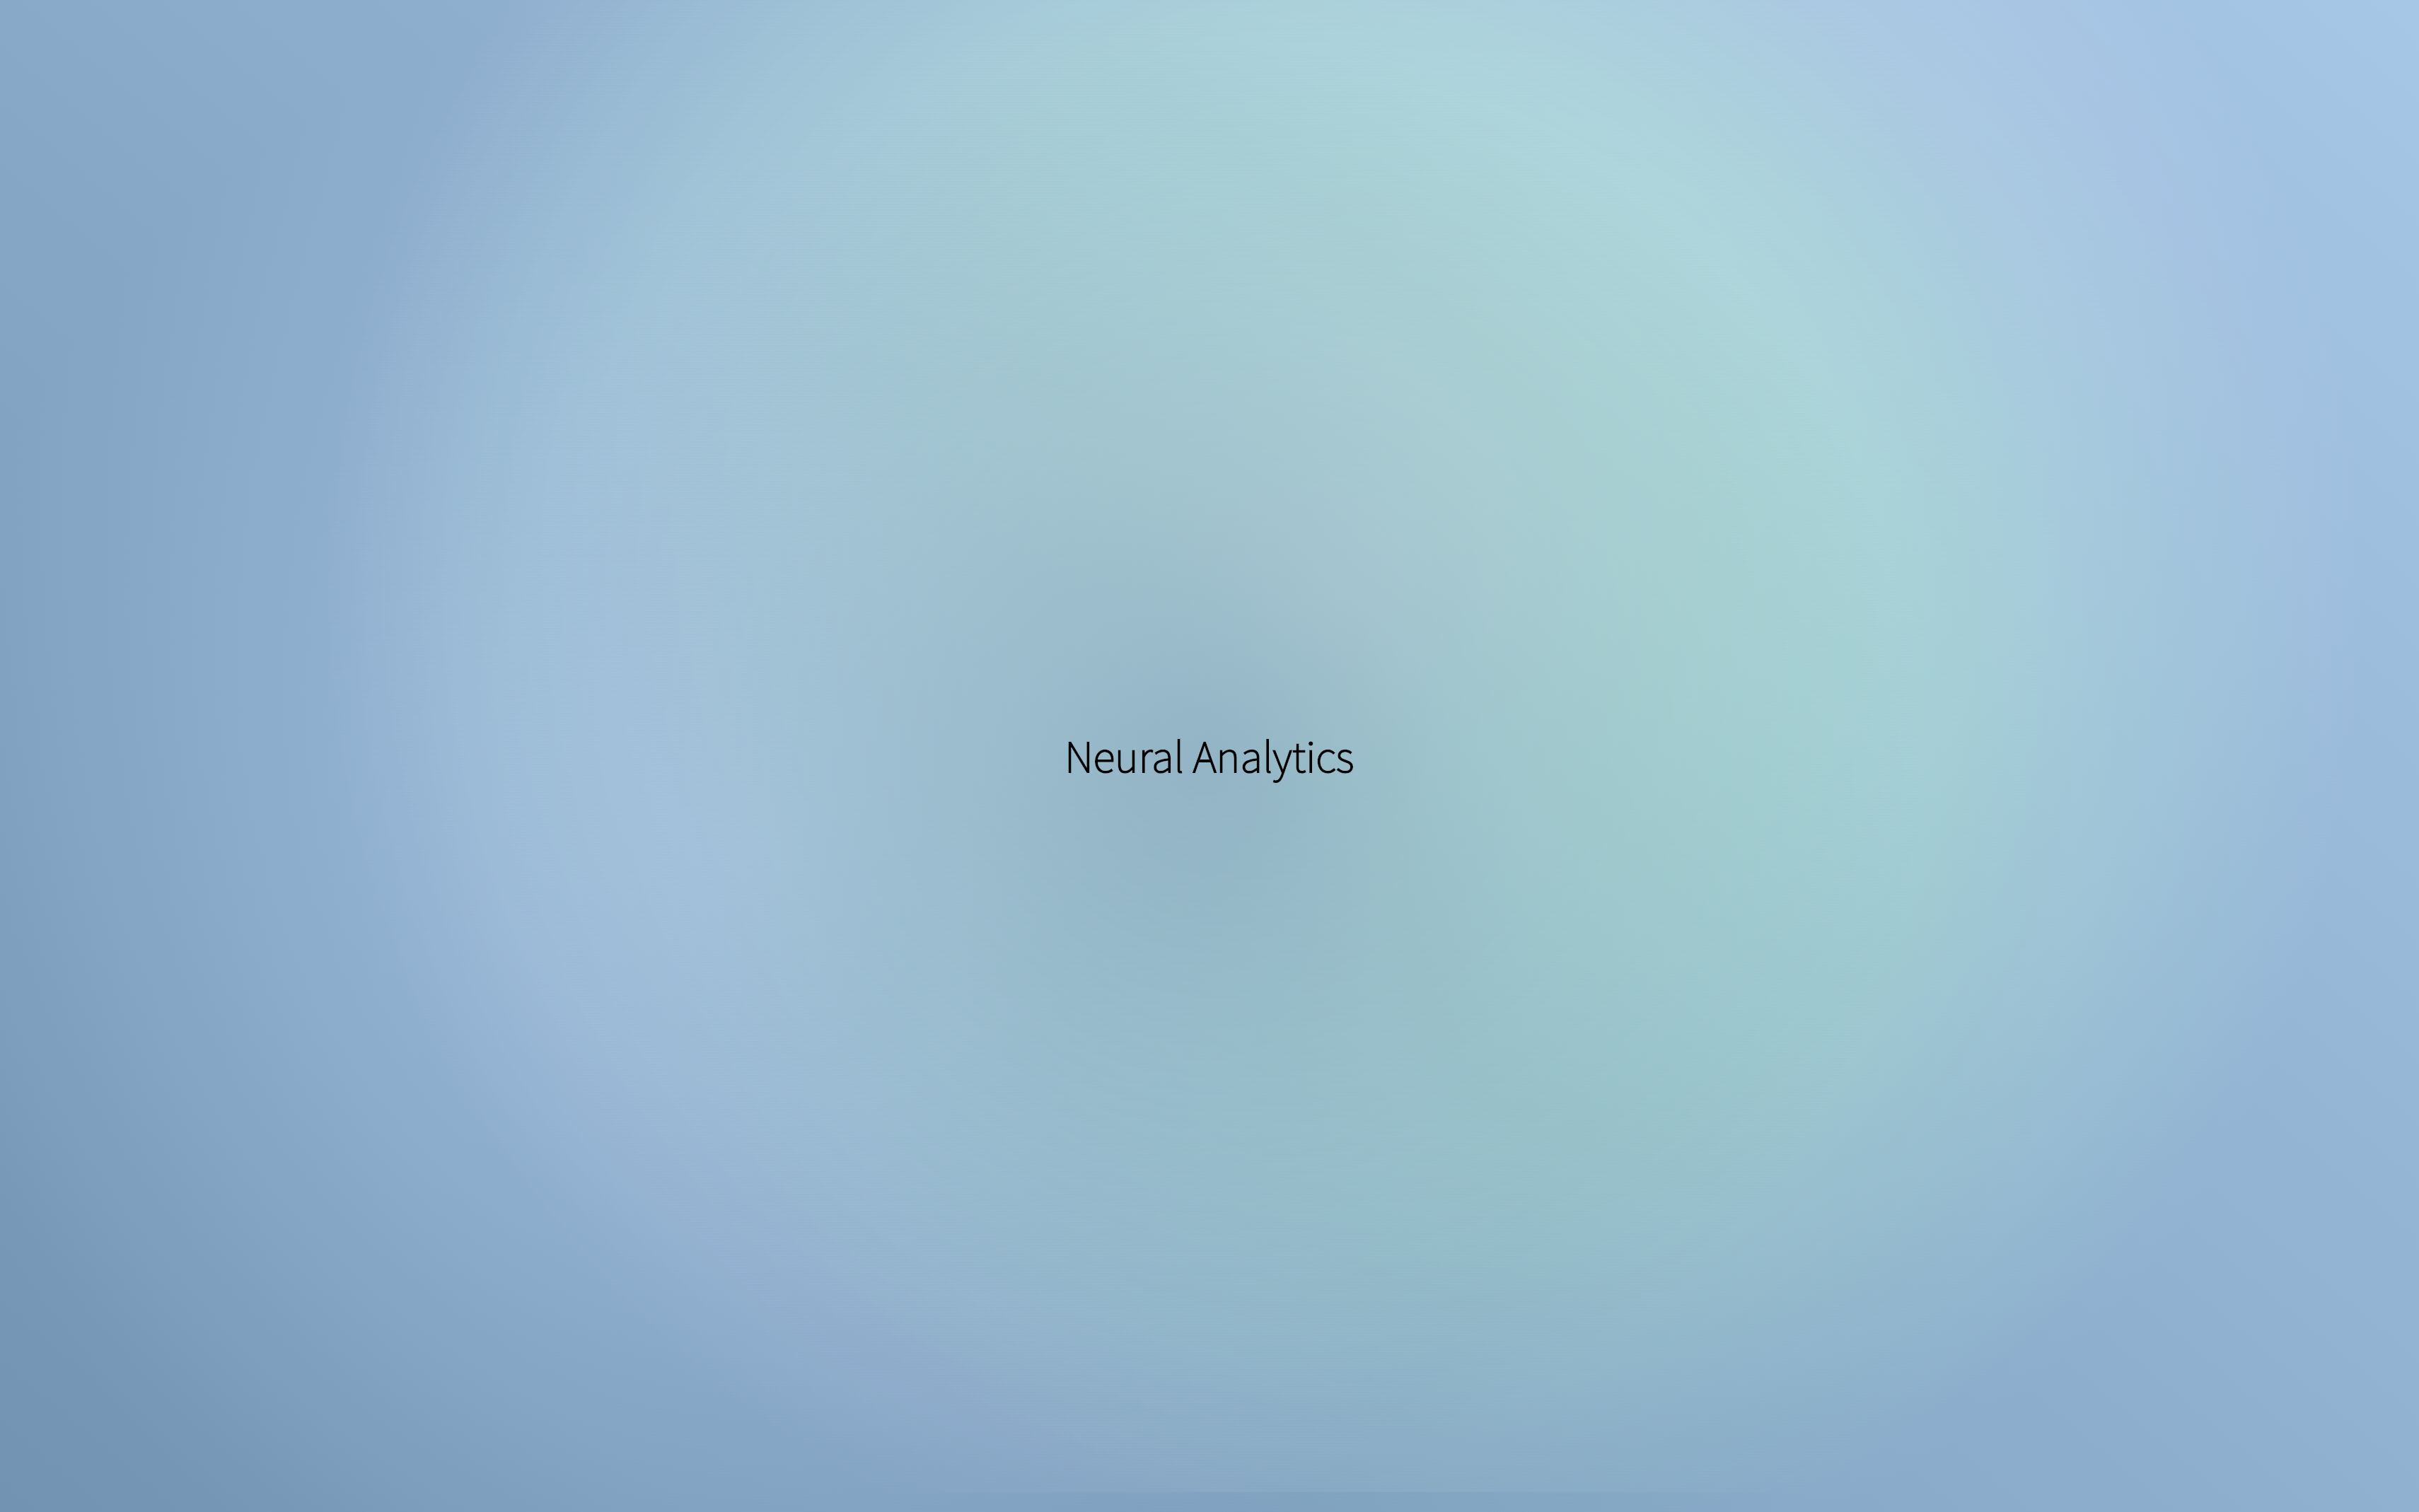
\includegraphics[width=0.7\textwidth]{assets/screenshots/inference/loading_app.png}
    \caption{Pantalla de carga inicial de la aplicación.}
\end{figure}

\section*{3. Pantalla de bienvenida}
Cuando la aplicación esté lista, aparecerá una pantalla que le pedirá encender la diadema EEG y colocársela correctamente. Siga la instrucción y espere a que el sistema lo detecte.

\begin{figure}[h!]
    \centering
    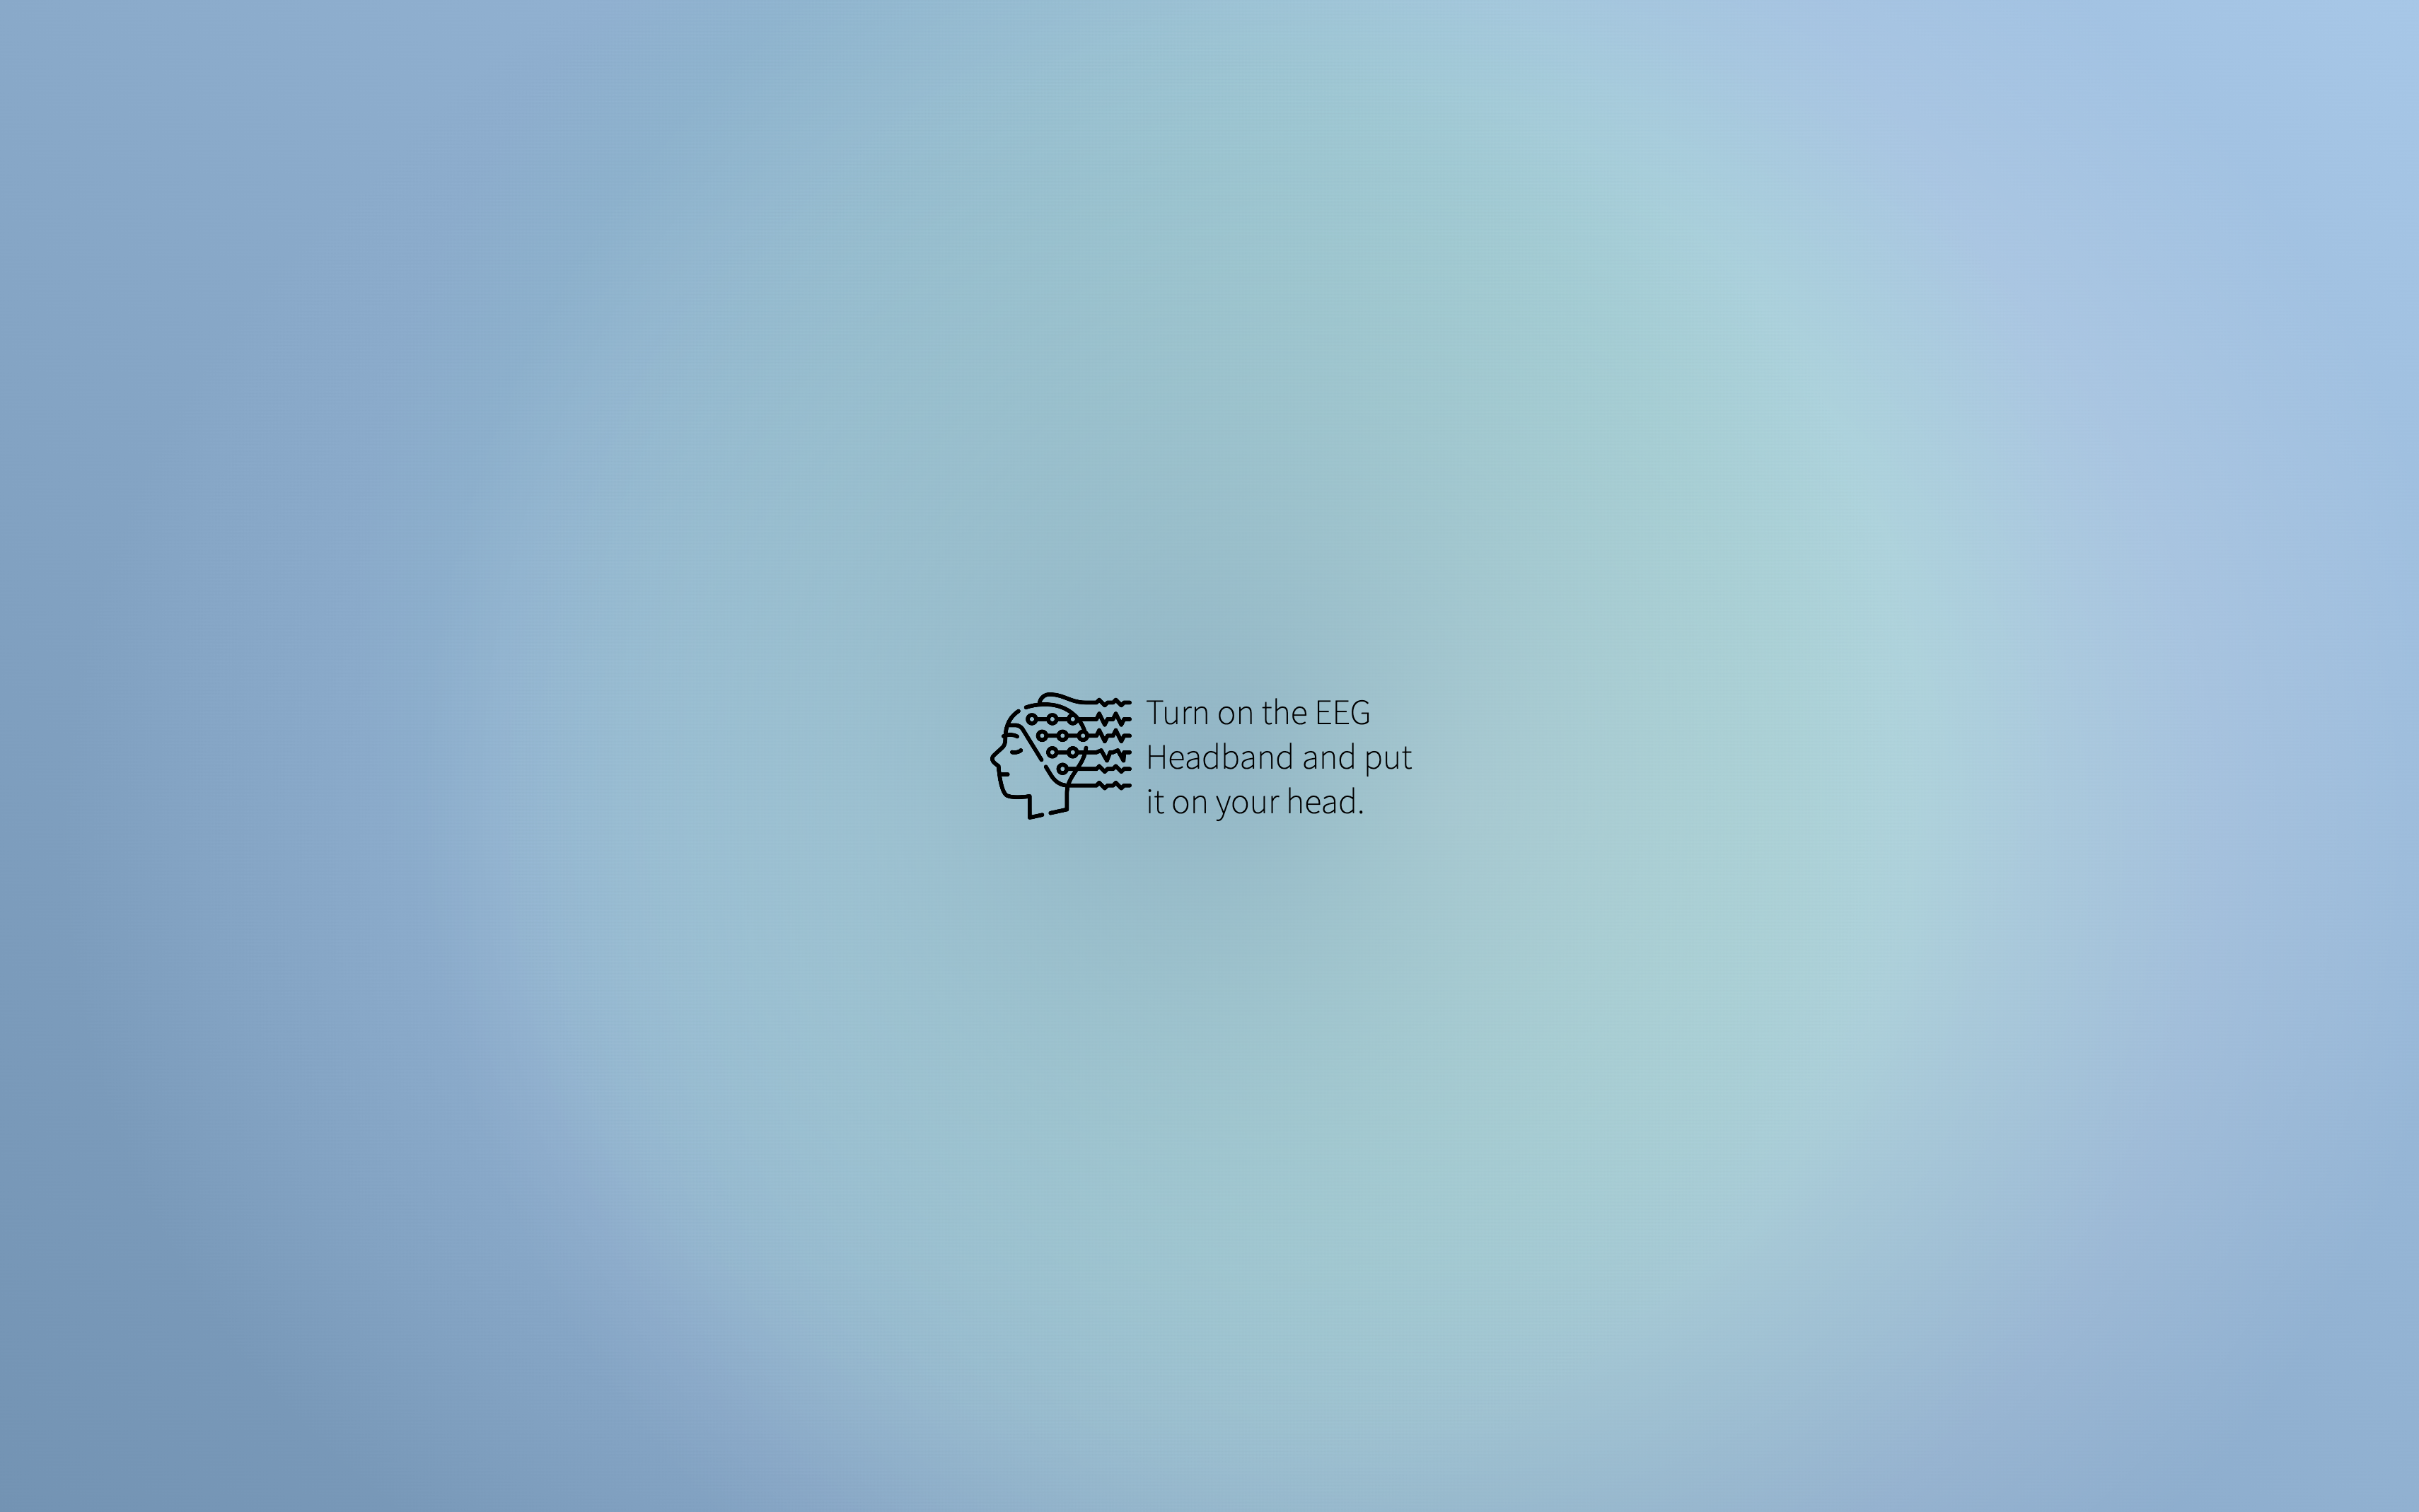
\includegraphics[width=0.7\textwidth]{assets/screenshots/inference/welcome_user.png}
    \caption{Pantalla de bienvenida e instrucciones para colocarse la diadema.}
\end{figure}

\section*{4. Calibración de electrodos}
Tras colocarse la diadema, la aplicación le guiará por una pantalla de calibración. Aquí podrá ver el estado de cada electrodo (T3, T4, O1, O2) mediante indicadores visuales (colores o iconos). Si algún electrodo aparece en rojo o con un símbolo de error, ajuste su posición hasta que todos estén en verde o con el símbolo de correcto.

\begin{figure}[h!]
    \centering
    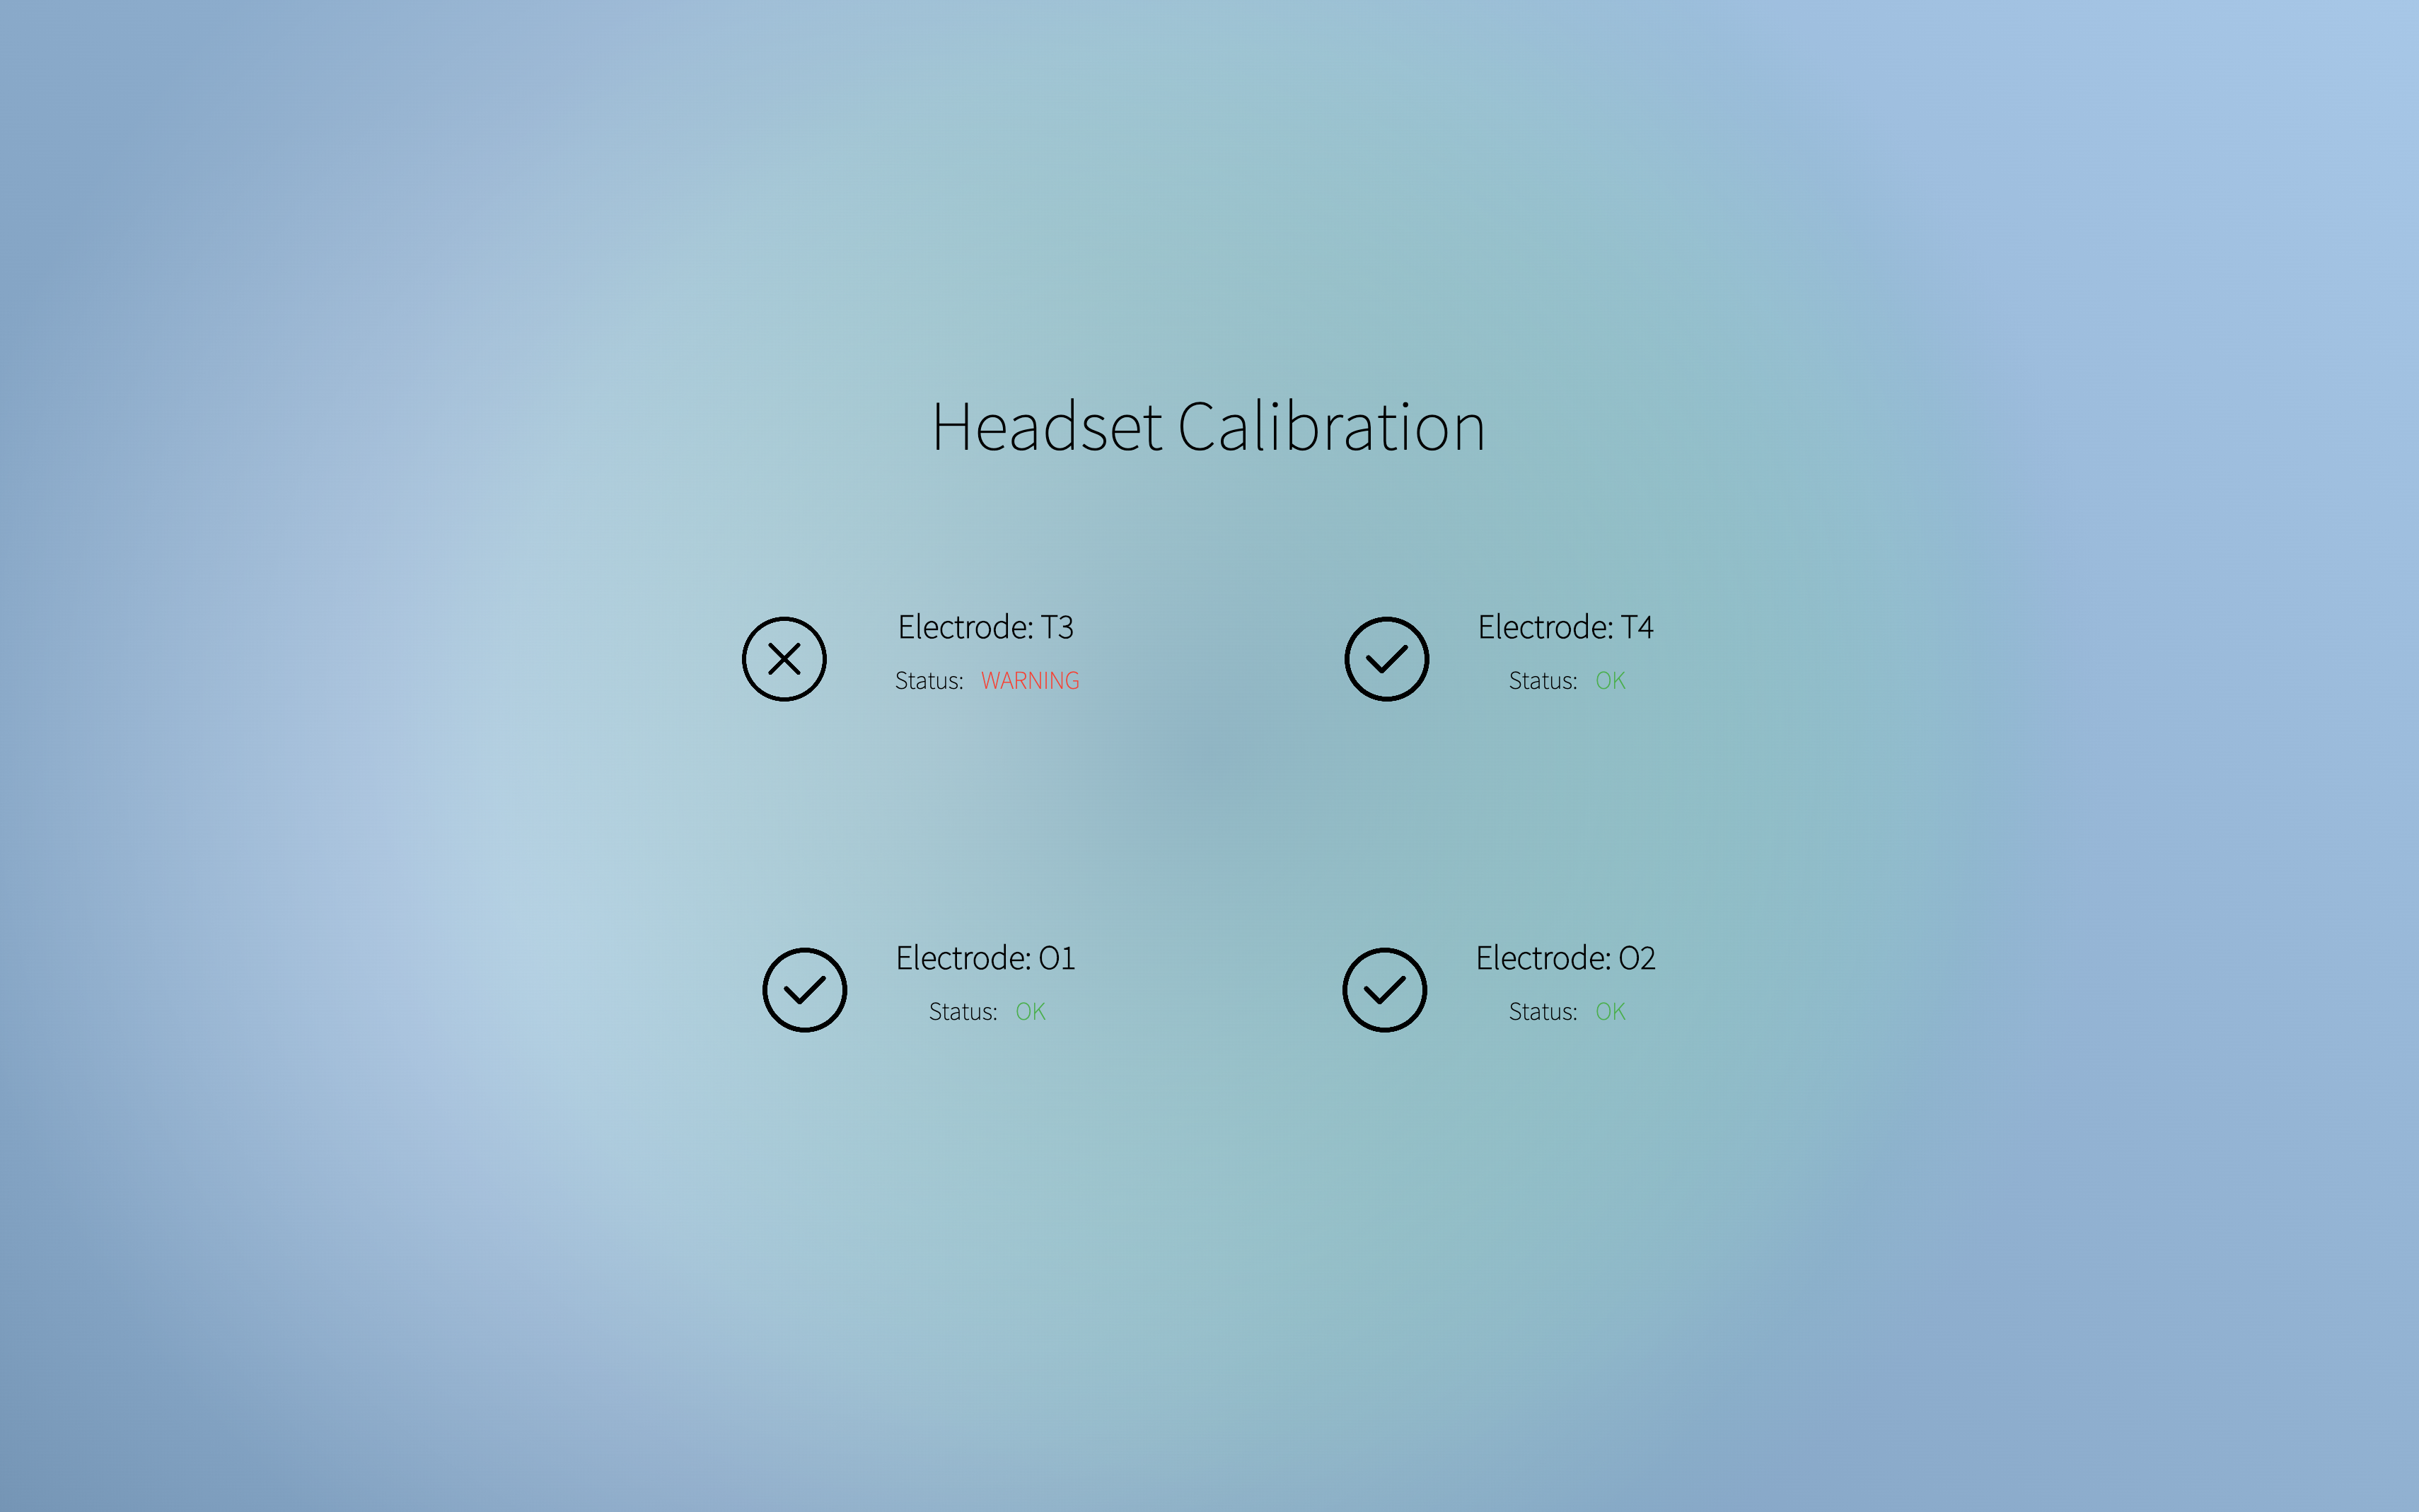
\includegraphics[width=0.7\textwidth]{assets/screenshots/inference/headset_calibration.png}
    \caption{Pantalla de calibración de electrodos.}
\end{figure}

\section*{5. Pantalla principal de inferencia}
Una vez calibrados los electrodos, accederá a la pantalla principal. Aquí podrá:
\begin{itemize}
    \item Ver en tiempo real las señales recogidas por cada electrodo, representadas en gráficas.
    \item Consultar el estado del sistema y el color de "pensamiento" detectado (por ejemplo, rojo o verde).
\end{itemize}

\begin{figure}[h!]
    \centering
    \includegraphics[width=0.8\textwidth]{assets/screenshots/inference/main_window.png}
    \caption{Pantalla principal de la aplicación de inferencia.}
\end{figure}

\section*{6. Mensajes y estados de la aplicación}
\begin{itemize}
    \item Si algún electrodo pierde contacto, la aplicación lo indicará y le pedirá ajustarlo.
    \item Si la señal es débil o hay interferencias, aparecerá un aviso. Siga las recomendaciones en pantalla.
    \item Si todo está correcto, los indicadores estarán en verde y podrá continuar.
    \item En caso de error grave, reinicie la aplicación y repita el proceso desde el inicio.
\end{itemize}

\section*{7. Consejos prácticos}
\begin{itemize}
    \item Coloque la diadema de forma cómoda y estable, evitando movimientos bruscos durante la sesión.
    \item Si ve que al usuario le aprieta mucho la banda para que sea conductiva, pruebe a mojar la cabeza del usuario con agua o gel para mejorar la conductividad.
    \item Si tiene dudas, consulte este manual o pida ayuda al responsable.
\end{itemize}


    \include{chapters/chapter_end/AlphabeticIndex}
\end{document}